% for sublime text 3
%!TEX root = diss.tex

\chapter{Related Work}
\label{ch:rel-work}
 
Coherence modeling has received a lot of attention due to its key impact in other natural language processing tasks. 
In this thesis, we propose a novel approach to local coherence modeling based on graph representations of texts. 
We apply our approach to two types of graphs. 
The first type captures corerfent relations between named entity mentions in a text.
The second one represents lexical relations between any word in a text.  
The impact of our coherence model is examined in readability assessment and text summarization. 

Accordingly, we first review entity-based approaches to local coherence (Section \ref{sec:rel-entity-models}). 
We then survey lexical approaches (Section \ref{sec:rel-ent-grid}). 
Finally, we discuss applications for local coherence model that have been introduced in the literature, particularly readability assessment and summarization tasks (Section \ref{sec:rel-coh-applications}). 
% A coherent text consists of a sequence of topics in a structured way \cite{marcu97b,hearst97,gallery03}. 
% Related models are often constructed as sequential topical models. 
% Topics are modeled by a language model \cite{blei01} or Bayesian topic models \cite{eisenstein08}.
% For modeling the temporal structure, early research uses a Hidden Markov Model \cite{barzilay04}, and  
% later research employs sequential neural networks \cite{}. 

\section{Entity-Based Approaches to Local Coherence}
\label{sec:rel-entity-models}

The primary steps of the research presented in this thesis is inspired by entity-based models. 
In this section, we explain details of two popular entity-based coherence models: the entity grid model, and the entity graph model. 
We also briefly discuss their extensions.  

\subsection{Historical Review}

Entity-based approaches to local coherence have a long history within the linguistic literature \cite{kuno72,halliday76,prince81a,joshi98}.
Most approaches are common in the primary assumption that coherence is perceived with respect to how entities are introduced and discussed in texts. 
At any point in a text, some entities are taken more salient than others, and consequently are supposed to manifest different properties. 
The main insight of entity-based models is that texts that keep referring to similar  entities are supposed to be more coherent than texts with random and unexpected switches from one entity to another. 
The primary underlying assumption is that the distributions of entities in coherent texts reveal certain regularities. 
This premise is supported by different theories, one of which is Centering Theory \cite{grosz95,joshi98} (see Chapter \ref{ch:coherence})

A great deal of research has been devoted to implement Centering Theory \cite{miltsakaki00,karamanis04a}. 
This is challenging because a computational model needs to determine how to instantiate parameters of the theory that are often underspecified. 
Interestingly, \newcite{poesio04} note that even for basic parameters of Centering Theory such as ``utterance'', ``realization'', and ``ranking'' (see Chapter \ref{ch:coherence}), multiple interpretations have been developed, because in the original theory of centering these concepts are not explicitly specified. 
As an instance, in some papers entities are ranked with respect to the grammatical function \cite{brennan87,grosz95} of entities occurrences in a text, and in some other papers those are ranked with respect to the position of entity mentions in sentences \cite{prince81a}, the familiarity status, or the thematic role \cite{strube.cl99,sidner04}.
As a result, two “instantiations” of the same theory make different predictions for the same input.  
Some studies aim to find an instantiation of parameters that is most consistent with observable data \cite{strube.cl99,karamanis04a,poesio04b}. 
Some others adopt a specific instantiation with the goal of improving the performance of the coherence model for a specific task. 
For example, \newcite{miltsakaki00} annotate a corpus of student essays with entity transition information, and then show that the distribution of transitions correlates with human grades. 
Analogously, \newcite{hasler04} investigates whether Centering Theory can be used in evaluating the readability of text by annotating human and machine generated summaries with the entity transition information. 
To sum up, \newcite{}Poesio et al. (2004) demonstrate that the predictive power of the centering theory is highly sensitive to its parameter definitions. 

One of the successful entity-based coherence frameworks, which is inspired by the Centering Theory, is the entity grid model \cite{barzilay05a,barzilay08}. 
This model uses the advantages of machine learning methods to encode patterns of entity distributions in texts.
Its main goal is to eliminate the need to human annotations for parameters in Centering Theory, regardless of what the evaluation task is. 

\subsection{The Entity Grid Model}
\label{sec:rel-ent-grid} 

\newcite{barzilay05a,barzilay08} were the first researchers who proposed a computational approach to local coherence modeling based on the entity relations among sentences. 
Supported by some linguistic work such as Centering Theory \cite{grosz95} and other entity-based theories of discourse \cite{givon87,prince81a}, they assume that the distribution of entities in locally coherent texts exhibits certain regularities that can be reflected in a grid topology that is called entity grid. 
In this thesis we refer to this model as the entity grid model, because its key idea is to represent a text as a grid that captures patterns of entity distributions across sentences in a text (see Chapter \ref{ch:coherence} for entity definition).  
In practice, mentions of an entity are linked together in order to show that they are referring to the same entity. 
Connections between mentions not only show that those are referring to the same entity, but also indicate that sentences that contain those mentions are (almost) about the same topic or information \cite{barzilay08}. 

\subsubsection{Text Representation: Entity Grid}

In the entity grid model each text is represented by a grid. 
A grid is a two dimensional array whose columns correspond to entities, and rows are matching to sentences.
An entry $r_{i;j}$ in a grid describes the syntactic role of entity $j$ in sentence $i$ if the entity is mentioned in the sentence. 
The syntactic roles are categorized as subject (S), object (O), or all other syntactic roles (X). 
In addition, if an entity is not mentioned in a sentence, a special marker (-) fills the corresponding entry $r_{i;j}$. 
Finally, if a sentence contains several mentions of one entity, their corresponding entry describes the most important grammatical role of the mentions: subject if possible, then object, or finally other. 

The discussion of the grid develops around the important question of which textual units are to be considered mentions of an entities, and how different mentions are to be linked to represent an entity. 
A perfect solution in this regard would use coreference resolution to recognize mentions, noun phrases, and link arbitrary mentions to the same entities and discarding noun phrases which do not correspond to an entity. 
Since coreference resolution systems are far from prefect\footnote{The highest reported precision of a coreference system on the ? dataset is ?.}, and tend to work even more poorly on incoherent texts, this approach is not generally one utilized \cite{barzilay05a}. 
Moreover, a non-perfect general coreference system introduces more noise to a coherence model than what it fixes \cite{barzilay08}.  
As an alternative, implementations of the entity grid tend to employ all noun phrases as mentions and perform a heuristic, but strict and simple, coreference resolution by connecting mentions that have an identical head noun as an entity. 
Detailed discussions of this heuristic are given in \newcite{poesio04c} and \newcite{elsner10}.

A sample text\footnote{The text with ID D31010, taken from Document Understanding Conference (DUC-?) dataset, which we use in one of our experiments. Numbers are not marked because they are filtered out in preprocessing.} is shown in Example \ref{ex:rel-text}. 
%/hits/fast/nlp/mesgarmn/Data/ACL13/SummaryCoherence/texts/
%D31010.M.100.T.E.txt. Nubembers (e.g. 29) are filtered out in preprocessing.}  


\begin{examples}
\label{ex:rel-text}
\begin{tabular}{l@{}p{12.5cm}}
 $S_0$: &[An arctic cold wave]\textbf{\textsubscript{S}}, [the worst]\textbf{\textsubscript{X}} in [10 years]\textbf{\textsubscript{X}}, hit [parts]\textbf{\textsubscript{O}} of [Europe]\textbf{\textsubscript{X}}, bringing [sub-zero temperatures]\textbf{\textsubscript{O}} and killing [scores]\textbf{\textsubscript{O}} of [people]\textbf{\textsubscript{X}}. \\

 $S_1$: & Hardest hit were [Poland]\textbf{\textsubscript{S}}, [Bulgaria]\textbf{\textsubscript{S}}, and [Romania]\textbf{\textsubscript{S}} as well as [parts]\textbf{\textsubscript{S}} of [central]\textbf{\textsubscript{X}} and [eastern France]\textbf{\textsubscript{X}}. \\

$S_2$: &In [Poland]\textbf{\textsubscript{X}}, [three weeks]\textbf{\textsubscript{X}} of [sub-zero temperatures]\textbf{\textsubscript{X}} killed [at least 85 people]\textbf{\textsubscript{O}} in [November]\textbf{\textsubscript{X}}, 29 more than in [all]\textbf{\textsubscript{X}} of [the previous winter]\textbf{\textsubscript{S}}. \\


$S_3$ : &[Most]\textbf{\textsubscript{S}} of [the victims]\textbf{\textsubscript{X}} were homeless [whose deaths]\textbf{\textsubscript{X}} by [exposure]\textbf{\textsubscript{X}} were alcohol related. \\

$S_4$: &[Blizzards]\textbf{\textsubscript{X}} and [cold temperatures]\textbf{\textsubscript{S}} also hit [Bulgaria]\textbf{\textsubscript{X}} and [Romania]\textbf{\textsubscript{O}}, stranding [hundreds]\textbf{\textsubscript{O}} in [their cars]\textbf{\textsubscript{X}}. \\

$S_5$: &Elsewhere, [snow]\textbf{\textsubscript{S}} blanketed [the Italian island]\textbf{\textsubscript{O}} of [Capri]\textbf{\textsubscript{X}} for [the first time]\textbf{\textsubscript{X}} in [10 years]\textbf{\textsubscript{X}}. 
\end{tabular}
\end{examples}

% \begin{examples}
% \label{ex:rel-text}
% \begin{center}
% \begin{tabular}{l@{\space}p{15cm}} %p@{\linewidth}
% \hline
%  $S_0$: & [An arctic cold wave]\textbf{\textsubscript{S}}, [the worst]\textbf{\textsubscript{X}} in [10 years]\textbf{\textsubscript{X}}, hit [parts]\textbf{\textsubscript{O}} of [Europe]\textbf{\textsubscript{X}}, bringing [sub-zero temperatures]\textbf{\textsubscript{O}} and killing [scores]\textbf{\textsubscript{O}} of [people]\textbf{\textsubscript{X}}. \\

%  $S_1$: & Hardest hit were [Poland]\textbf{\textsubscript{S}}, [Bulgaria]\textbf{\textsubscript{S}}, and [Romania]\textbf{\textsubscript{S}} as well as [parts]\textbf{\textsubscript{S}} of [central]\textbf{\textsubscript{X}} and [eastern France]\textbf{\textsubscript{X}}. \\

% $S_2$: & In [Poland]\textbf{\textsubscript{X}}, [three weeks]\textbf{\textsubscript{X}} of [sub-zero temperatures]\textbf{\textsubscript{X}} killed [at least 85 people]\textbf{\textsubscript{O}} in [November]\textbf{\textsubscript{X}}, 29 more than in [all]\textbf{\textsubscript{X}} of [the previous winter]\textbf{\textsubscript{S}}. \\


% $S_3$ : & [Most]\textbf{\textsubscript{S}} of [the victims]\textbf{\textsubscript{X}} were homeless [whose deaths]\textbf{\textsubscript{X}} by [exposure]\textbf{\textsubscript{X}} were alcohol related. \\

% $S_4$: & [Blizzards]\textbf{\textsubscript{X}} and [cold temperatures]\textbf{\textsubscript{S}} also hit [Bulgaria]\textbf{\textsubscript{X}} and [Romania]\textbf{\textsubscript{O}}, stranding [hundreds]\textbf{\textsubscript{O}} in [their cars]\textbf{\textsubscript{X}}. \\

% $S_5$: & Elsewhere, [snow]\textbf{\textsubscript{S}} blanketed [the Italian island]\textbf{\textsubscript{O}} of [Capri]\textbf{\textsubscript{X}} for [the first time]\textbf{\textsubscript{X}} in [10 years]\textbf{\textsubscript{X}}.  \\
% \hline
% \end{tabular}
% \end{center}
% % \caption{/hits/fast/nlp/mesgarmn/Data/ACL13/SummaryCoherence/texts/D31010.M.100.T.E.txt. Nubembers (e.g. 29) are filtered out in preprocessing.}
% \end{examples}

%%(ROOT (S (NP (NP (DT An) (JJ arctic) (JJ cold) (NN wave)) (, ,) (NP (NP (DT the) (JJS worst)) (PP (IN in) (NP (CD 10) (NNS years)))) (, ,)) (VP (VBD hit) (NP (NP (NNS parts)) (PP (IN of) (NP (NNP Europe)))) (, ,) (S (VP (VP (VBG bringing) (NP (JJ sub-zero) (NNS temperatures))) (CC and) (VP (VBG killing) (NP (NP (NNS scores)) (PP (IN of) (NP (NNS people)))))))) (. .)))

%%(ROOT (S (S (VP (ADVP (RBS Hardest)) (VBN hit))) (VP (VBD were) (NP (NP (NP (NNP Poland)) (, ,) (NP (NNP Bulgaria)) (, ,) (CC and) (NP (NNP Romania))) (CONJP (RB as) (RB well) (IN as)) (NP (NP (NNS parts)) (PP (IN of) (NP (NP (JJ central)) (CC and) (NP (JJ eastern) (NNP France))))))) (. .)))

%%(ROOT (S (PP (IN In) (NP (NNP Poland))) (, ,) (NP (NP (CD three) (NNS weeks)) (PP (IN of) (NP (JJ sub-zero) (NNS temperatures)))) (VP (VBD killed) (NP (QP (IN at) (JJS least) (CD 85)) (NNS people)) (PP (IN in) (NP (NNP November))) (, ,) (PP (ADVP (NP (CD 29)) (RBR more)) (IN than) (IN in) (NP (NP (DT all)) (PP (IN of) (NP (DT the) (JJ previous) (NN winter)))))) (. .)))

%%(ROOT (S (NP (NP (JJS Most)) (PP (IN of) (NP (DT the) (NNS victims)))) (VP (VBD were) (ADJP (JJ homeless) (SBAR (WHNP (NP (WP$ whose) (NNS deaths)) (PP (IN by) (NP (NN exposure)))) (S (VP (VBD were) (ADJP (RB alcohol) (VBN related))))))) (. .)))

%%(ROOT (S (NP (NP (NNS Blizzards)) (CC and) (NP (JJ cold) (NNS temperatures))) (ADVP (RB also)) (VP (VBD hit) (NP (NNP Bulgaria) (CC and) (NNP Romania)) (, ,) (S (VP (VBG stranding) (NP (NNS hundreds)) (PP (IN in) (NP (PRP$ their) (NNS cars)))))) (. .)))

%%(ROOT (S (ADVP (RB Elsewhere)) (, ,) (NP (NN snow)) (VP (VBD blanketed) (NP (NP (DT the) (JJ Italian) (NN island)) (PP (IN of) (NP (NNP Capri)))) (PP (IN for) (NP (NP (DT the) (JJ first) (NN time)) (PP (IN in) (NP (CD 10) (NNS years)))))) (. .)))
%%


\begin{table}
\centering
\begin{tabular}{lcccccc}
\hline
WAVE & S & - & - & - & - & - \\
WORST & X & - & - & - & -  &- \\
YEARS  &X  & -  &-  &-  &-  &X \\
PARTS  &O & S  &-  &-  &-  &-  \\
EUROPE  &X & - & - & - & - & - \\
TEMPERATURES  &O  &-  &X  &-  &S  &-  \\
SCORES  &O  &-  &-  &-  &-  &-  \\
PEOPLE  &X  &- & O  &-  &-  &-  \\
POLAND  &-  &S & X  &-  & -  &-  \\
BULGARIA  &-  &S  &-  &-  &X  &-  \\
ROMANIA  &-  &S  &-  &-  &O  &-  \\
CENTRAL  &-  &X  &- & - & - & -  \\
FRANCE  &-  &X  &-  &- & - & -  \\
NOVEMBER  &-  &- & X  &-  &-  &-  \\
WEEKS  &-  &-  &S  &-  &-  &-  \\
ALL  &-  &-  &X  &-  &-  &-  \\
WINTER  &-  & -  &X  &-  &-  &-  \\
MOST  &-  &-  &-  &S  &- & -  \\
VICTIMS  &-  &-  &-  &X  &-  &-  \\
DEATHS  &-  &-  &- & X  &-  &-  \\
EXPOSURE  &- & - & -  &X  &-  &-  \\
ALCOHOL  &-  &-  &-  &X  &-  &-  \\
BLIZZARDS  &-  &-  &-  &-  &X  &-  \\
HUNDREDS  &-  &-  &-  &-  &O  & -  \\
CARS  &-  &-  &-  &-  &X  &-  \\
TIME  &-  &-  &-  &-  &-  &X  \\
SNOW  &-  &- & - & - & - & S  \\
ISLAND & - & - & - & - & - & O  \\
CAPRI & - & - & - & - & - & X  \\
\hline
\end{tabular}
\caption{/hits/fast/nlp/mesgarmn/Data/ACL13/SummaryCoherence/NounGrid/SCR/wo\_coref/D31010.M.100.T.E.txt.grid. Mentions are head of NPs.}
\end{table}

\cite{elsner11a} show that adding non-head nouns to a grid is beneficial to improve the representation power of the entity grid model. 
By doing this, the model is able to pick up not only head nouns but pre-modifiers in noun phrases, like "the personal \textbf{country} flight". 
In the original version of the entity grid representation, mentions are indicated by head of NPs (\emph{flight} in this example) whereas the Elsner's extension considers all nouns (both \emph{country},\emph{flight} in the above example). 
The non-head mentions are given the role X. 

\subsection{Pattern Extraction: Grammatical Transitions}
%
The core hypothesis in the entity grid model is that grammatical transitions of entities reveal similar patterns in coherent texts. 
\newcite{barzilay05a} models these patterns by means of all possible ways that grammatical roles of entities changes over adjacent sentences. 
A sequence of employed grammatical symbols with size $n$, $\left \{S,O,X,\-–\right \}^n$, represents a pattern that encodes entity occurrences between sentences and the way that their syntactic roles in $n$ adjacent sentences are changing. 
For instance, for two adjacent sentences ($n=2$) there are $16$ possible patterns for syntactical transitions of entities, defined as below:

\begin{equation}
S S\textit{, }S O\textit{, } S X\textit{, } S \textit{ --, }  O S\textit{, }O O\textit{, }O X\textit{, }  O \textit{ --, }  X S\textit{, }  X O\textit{, }  X X\textit{, } X \textit{ --, -- }S\textit{, -- }O\textit{, -- }X\textit{, -- --}  
\end{equation}
%
where each encodes one possible way of syntactical transition of an entity between two adjacent sentences. 

\subsubsection{Coherence Representation: Probabilities of Transitions}
%
The frequency of predefined grammatical transitions is an indicator to the preference of coherent texts in using or avoiding certain transitions. 
Inspired by the Centering Theory, coherent texts may reveal certain regularities over the frequencies or probabilities of these patterns. 
Given an entity grid representation of a text, the probability of each of grammatical transitions is computed as follows:

\begin{equation}
P(t) = \frac{n(t)}{n(t^*)},
\end{equation}
where $t$ is a transition of grammatical roles, $n(t)$ indicates the number of times that this transition is occurring in the entity grid, the denominator or $n(t^*)$ depicts the number of all transitions with the same length as the length of $t$. 
Table \ref{} shows an example of a feature vector text representation using all transitions of length two given syntactic categories \textbf{S},\textbf{O},\textbf{X}, and \textbf{-}.

\begin{table}
\centering
\begin{tabular}{@{}cccccccccccccccc@{}}
\hline
S S & S O  & S X & S -- & O S  & O O  & O X  & O -- & X S  & X O  & X X & 	X -- & -- S  & -- O  & -- X & -- -- \\\hline
$.00$ & $.01$  & $.02$ & $.01$  & $.00$  & $.01$  & $.04$  & $.01$  & $.01$  & $.01$  & $.04$ & $.05$  & $.02$  & $.02$  & $.02$ & $.72$ \\
\hline
\end{tabular}
\caption{}
\end{table}


Centering Theory and its extensions try to linguistically define and rank patterns with respect to human annotations, and final evaluation task. 
The key advantage of the entity grid representation of a text is that the probability of these patterns can be simply computed and
the coherence property of a text can be encoded by a vector whose elements are probabilities of the transition patterns. 
These probabilities are coherence features and the vector of them is a feature vector representing the coherence of a text. 
Given a dataset consisting of texts with different ranks of coherence, the above model encodes each text by its coherence feature vector.  
These vectors can be utilized by machine learning algorithms to distinguish texts with respect to their coherence property. 
As a result this model automatically learns to learn patterns.

\subsubsection{Extensions}
%
Several extensions of the entity grid model have been proposed. 
Most of them define different strategies for mention detections and their grouping in entities. 

\newcite{filippova.enlg07} extend the entity gird approach on coherence modeling from coreference to semantic relatedness. 
They show that by grouping related entities the performance of the entity grid improves, especially when syntactical information of entities are not involved. 
To do this, they use WikiRelate \cite{strube.aaai06} to compute relatedness between entities, $SemRel(e_i,e_j) >t$, where $t$ is a threshold.
Different values of $t$ results in different grid density, the smaller the value, the denser the grid but the less related words within one entity group are. 
They show that using semantic relatedness between entities improve the the performance of the original entity grid model.  
However, semantic clustering of entities on top of coreference grouping did not bring an improvement. 

\newcite{elsner08b} uses information status (New or first mention vs Given or subsequent) of the entities, rather than their syntactical roles. 
They run a maximum-entropy classifier to detect each noun phrase, NP, as a label $L_{np} \in \lbrace new, old \rbrace$. 
The coherence score of a document is then estimated by multiplication of probabilities of information status of each mention. 
They show that adding a discourse-new classifier, which distinguishes discourse-new entities from -old ones, improve the performance of the entity grid model. 
Another finding of this paper is that, just using a pronoun resolution system in entity definition enhances the entity grid representation and the quality of the coherence model. 
Indeed, although the coreference systems are far away from prefect, pronoun resolution systems as a highly precise (but specific) coreference system can be used to have more meaningful entities. 

\newcite{elsner11b} extend the entity grid representation by adding other information about entities such as named entity type, entity importance using coreference features (e.g., Is\_Named\_entity, Has\_Singular\_Mention, Has\_Proper\_Mention, etc). 
They motivate their work in this way that distinguishing important from unimportant entity types is important in applications such as coreference \cite{haghighi10} and summarization \cite{nenkova05}. 
Therefore, adding current context information of entities will improve the performance of the entity grid model. 


\newcite{linziheng11a} assume that a coherent text has certain discourse relation patterns. 
Instead of modeling entity transitions, they model discourse role transitions between sentences.
In a follow up work, \newcite{feng14} train the same model but using features derived from deep discourse structures annotated with Rhetorical Structure Theory or RST relations \cite{mann88}. 

\newcite{louis12} introduced a coherence model based on syntactic patterns in text by assuming that sentences in a coherent discourse should share the same structural syntactic patterns.

% \newcite{louis12} models the coherence between adjacent sentences by a hidden Markov framework where captures the transition rules of different topics.


\newcite{joty17} (acl17) proposed a deep learning version of the entity grid model. 
Their model first transforms the grammatical roles in an entity grid into their vector representations, and employs a convolution operation over it to model entity transitions in the distributed space. 
The spatially max-pooled features from the convoluted features are used for coherence scoring. 
In a latter work, \newcite{joty18} (ACL18) extend their neural entity grid model by lexicalizing its entity transitions such that each entry of the entity grid contains two vectors, one representing its corresponding entity and one representing the grammatical role of the entity in the corresponding sentence.  


% In practice, most implementations follow \newcite{barzilay05} are conditioning on a measure of
% salience, which ideally should measure the importance of a particular entity to the document. 
% The intuition is that the effect of the transition of prominent entities affect the coherence of a text more than transitions of the other entities. 
% The usual way of representing this is to condition on the number of times the entity occurs throughout the text.

To conclude this part, we point out pros and cons of the entity grid representation and model. 
The prominent benefit of the entity grid model is that it can learn the properties of coherent texts, which is based on the patterns of entity distributions, from a corpus, without recourse to manual annotation or a predefined knowledge base.
The main weakness of the entity grid model, namely is its disability to describe global topical structure or lexical co-occurrences because it is defined over adjacent sentences. 
Although the sequence's length of grammatical transitions, $n$, can be large, in practice it has not been set more than $2$. 
The reason is that with longer sequences, the number of possible coherence features increases yielding sparse feature vectors. 
Moreover, by increasing the length of sequences, the model does not incorporate the relations between non-adjacent sentences that occur in well-written texts. 


\subsection{The Entity Graph Model}
\label{sec:ent_graph}
%
The entity graph \cite{guinaudeau13} model provides a graph-based representation for modeling the distribution of entities across sentences. 
Graphs are a more powerful representation for coherence than then the grid representation  \cite{barzilay08}, because it is restricted to transitions between adjacent sentences; whereas graphs can span the entire text.  
In contrast to the entity grid representation that contains information about absent entities (grammatical  transitions that contain $--$ $--$), the graph-based representation only take information of present entities in sentences into account.  

Another advantage of graph-based methods is that, once a problem is formulated as a graph problem, then existing standard solutions in graph theories can be used to solve the problem. 

\subsubsection{Text Representation: Entity Graph}
%

The key idea is that the entity grid representation \cite{barzilay08} can be interpreted as the adjacency matrix of a bipartite graph representing  sentences, entities and their connections in a text. 
Then, appropriate properties and algorithms of graph theory model the connectivity of entity graphs and consequently the coherence of the text. 

The entity grid representation is restricted to connections between adjacent sentences. 
It does not model the long distant entity connections between sentences. 
The entity grid representation also captures the absence of entity connections between sentences. 
Encoding this information results in sparse matrix representations of texts. 
Patterns without any syntactical roles (e.g. $-- --$) obtains higher probability in comparison with other patterns, because they are frequent in all matrices. 

Graph representation is a suitable solution to overcome these limitations. 
Graphs let easily encode long distance links in a text. 
They also only connect two nodes if there is a relation between them, and does not capture beneficial entities. 

The entity graph considers the entity grid representation of a text as the incidence matrix of a bipartite graph that represent the distribution of entities over sentences of a text. 
Each node of a graph represents either a sentence or an entity of a text. 
A bipartite graph, in general, is a graph with two independent sets of nodes.
Entity graph assigns a set of nodes to sentences and a set node to entities in a text.
Edges in bipartite graph connect only a node of sentence nodes to a node of the entity nodes, and each edge represents that a mention of the associated entity to the entity node exists in the associated sentence to the sentence node.  
This is equivalent with entries in the entity grid representation that are not equal to ``--''. 
The grammatical role of an entity in a sentence is encoded in the entity graph by a weight of the edge that connects the entity node to the sentence node. 
Given the linguistic intuition that entities with important syntactical roles are prominent entities in each sentence, the entity graph model simply assigns three numbers $3>2>1$ to model subject (S), object (O), and any others syntactical roles (X) represented in the entity grid. 

Entity graph model is established on the entity grid representation of a text. 
Therefore, the way of obtaining entities in the entity grid representation affects the performance of the entity grid model as well.  
Similar to \newcite{elsner11b}, \newcite{guinaudeau13} take all nouns in a text as mentions of entities, even those that are not head of any noun phrase. 

Figure \ref{fig:entity_graph} depicts the entity graph representation of the text in example \ref{}.

\begin{figure}[!ht]
\centering
\small
\begin{tabular}{c}

 %%%%%%%%%%%%%%%%%%%%%%%%%%%%%% bipartite graph for : wsj_1818%%%%%%%%%%%%%%%%%%%%%%%%%%%%%%
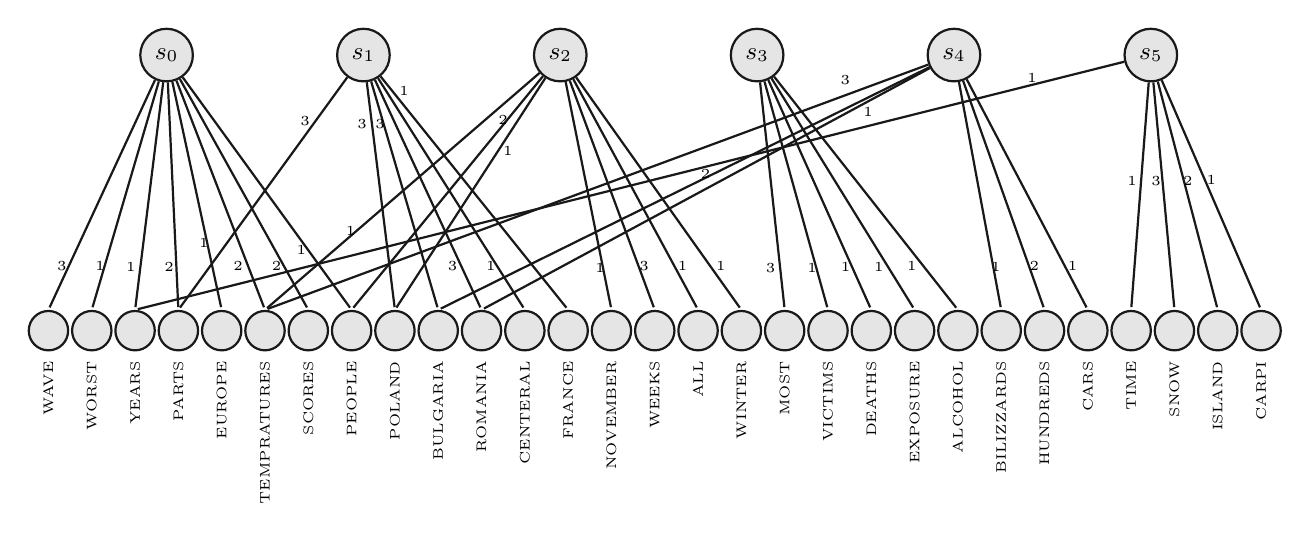
\begin{tikzpicture}[shorten >=1pt,-,scale=0.5]  
		\tikzstyle{sentence}=[circle,thick,draw=black!90,fill=black!10,minimum size=2mm]
	\tikzstyle{entity}=[circle,thick,draw=black!90,fill=black!10,minimum size=5mm]
		\tikzstyle{edge}=[draw=black!90, thick]
	   \begin{scope}
	   
		 \node [sentence] (s0) at (-3,0) {\small{$s_0$}};
		 \node [sentence] (s1) at (2,0) {\small{$s_1$}};
		 \node [sentence] (s2) at (7,0) {\small{$s_2$}}; 
		 \node [sentence] (s3) at (12,0) {\small{$s_3$}}; 
		 \node [sentence] (s4) at (17,0) {\small{$s_4$}};
		 \node [sentence] (s5) at (22,0) {\small{$s_5$}}; 
		 


	 \node [entity, label=below:\rotatebox{+90}{\tiny{WAVE}}] (e0)  at (-6.0,-7) {}; 
	 \node [entity, label=below:\rotatebox{+90}{\tiny{WORST}}] (e1)  at (-4.9,-7) {};
	 \node [entity, label=below:\rotatebox{+90}{\tiny{YEARS}}] (e2)  at (-3.8,-7) {}; 
	 \node [entity, label=below:\rotatebox{+90}{\tiny{PARTS}}] (e3)  at (-2.7,-7) {}; 
	 \node [entity, label=below:\rotatebox{+90}{\tiny{EUROPE}}] (e4)  at (-1.6,-7) {}; 
	 \node [entity, label=below:\rotatebox{+90}{\tiny{TEMPRATURES}}] (e5)  at (-0.5,-7) {}; 
	 \node [entity, label=below:\rotatebox{+90}{\tiny{SCORES}}] (e6)  at (0.6,-7) {}; 
	 \node [entity, label=below:\rotatebox{+90}{\tiny{PEOPLE}}] (e7)  at (1.7,-7) {}; 
	 \node [entity, label=below:\rotatebox{+90}{\tiny{POLAND}}] (e8)  at (2.8,-7) {}; 
	 \node [entity, label=below:\rotatebox{+90}{\tiny{BULGARIA}}] (e9)  at (3.9,-7) {}; 
	 \node [entity, label=below:\rotatebox{+90}{\tiny{ROMANIA}}] (e10)  at (5.0,-7) {}; 
	 \node [entity, label=below:\rotatebox{+90}{\tiny{CENTERAL}}] (e11)  at (6.1,-7) {}; 
	 \node [entity, label=below:\rotatebox{+90}{\tiny{FRANCE}}] (e12)  at (7.2,-7) {}; 
	 \node [entity, label=below:\rotatebox{+90}{\tiny{NOVEMBER}}] (e13)  at (8.3,-7) {}; 
	 \node [entity, label=below:\rotatebox{+90}{\tiny{WEEKS}}] (e14)  at (9.4,-7) {}; 
	 \node [entity, label=below:\rotatebox{+90}{\tiny{ALL}}] (e15)  at (10.5,-7) {}; 
	 \node [entity, label=below:\rotatebox{+90}{\tiny{WINTER}}] (e16)  at (11.6,-7) {}; 
	 \node [entity, label=below:\rotatebox{+90}{\tiny{MOST}}] (e17)  at (12.7,-7) {}; 
	 \node [entity, label=below:\rotatebox{+90}{\tiny{VICTIMS}}] (e18)  at (13.8,-7) {}; 
	 \node [entity, label=below:\rotatebox{+90}{\tiny{DEATHS}}] (e19)  at (14.9,-7) {}; 
	 \node [entity, label=below:\rotatebox{+90}{\tiny{EXPOSURE}}] (e20)  at (16.0,-7) {}; 
	 \node [entity, label=below:\rotatebox{+90}{\tiny{ALCOHOL}}] (e21)  at (17.1,-7) {}; 
	 \node [entity, label=below:\rotatebox{+90}{\tiny{BILIZZARDS}}] (e22)  at (18.2,-7) {}; 
	 \node [entity, label=below:\rotatebox{+90}{\tiny{HUNDREDS}}] (e23)  at (19.3,-7) {}; 
	 \node [entity, label=below:\rotatebox{+90}{\tiny{CARS}}] (e24)  at (20.4,-7) {}; 
	 \node [entity, label=below:\rotatebox{+90}{\tiny{TIME}}] (e25)  at (21.5,-7) {}; 
	 \node [entity, label=below:\rotatebox{+90}{\tiny{SNOW}}] (e26)  at (22.6,-7) {}; 
	 \node [entity, label=below:\rotatebox{+90}{\tiny{ISLAND}}] (e27)  at (23.7,-7) {}; 
	 \node [entity, label=below:\rotatebox{+90}{\tiny{CARPI}}] (e28)  at (24.8,-7) {}; 

		 
	 \path[edge] (s0) edge [above, very near end] node[font=\tiny] {$3$} (e0.north); %, line width=0.3ex
	 \path[edge] (s0) edge [above, very near end] node[font=\tiny] {$1$} (e1.north);
	 \path[edge] (s0) edge [above, very near end] node[font=\tiny, xshift=-1mm] {$1$} (e2.north);
	 \path[edge] (s0) edge [above, very near end] node[font=\tiny, xshift=-1mm] {$2$} (e3.north);
	 \path[edge] (s0) edge [above, very near end] node[font=\tiny, yshift=3mm, xshift=-1.5mm] {$1$} (e4.north);
	 \path[edge] (s0) edge [above, very near end] node[font=\tiny, xshift=-2mm] {$2$} (e5.north);
	 \path[edge] (s0) edge [above, very near end] node[font=\tiny, xshift=-2mm] {$2$} (e6.north);
	 \path[edge] (s0) edge [above, very near end] node[font=\tiny, yshift=2mm, xshift=-3.7mm] {$1$} (e7.north);

	 \path[edge] (s1) edge [above, near start] node[font=\tiny, near start] {$3$} (e3.north);
	 \path[edge] (s1) edge [above, near start] node[font=\tiny, xshift=-1.5mm] {$3$} (e8.north);
	 \path[edge] (s1) edge [above, near start] node[font=\tiny, xshift=-1mm] {$3$} (e9.north);
	 \path[edge] (s1) edge [above, very near end] node[font=\tiny, xshift=-2mm] {$3$} (e10.north);
	 \path[edge] (s1) edge [above, very near end] node[font=\tiny, xshift=-2mm] {$1$} (e11.north);
	 \path[edge] (s1) edge [above, very near start] node[font=\tiny] {$1$} (e12.north);

	 \path[edge] (s2) edge [above, very near end] node[font=\tiny, yshift=4.4mm, xshift=6.5mm] {$1$} (e5.north);
	 \path[edge] (s2) edge [above, near start] node[font=\tiny, xshift=1mm] {$2$} (e7.north);
	 \path[edge] (s2) edge [below, near start] node[font=\tiny] {$1$} (e8.north);
	 \path[edge] (s2) edge [below,  near end] node[font=\tiny] {$1$} (e13.north);
	 \path[edge] (s2) edge [above, very near end] node[font=\tiny] {$3$} (e14.north);
	 \path[edge] (s2) edge [above, very near end] node[font=\tiny] {$1$} (e15.north);
	 \path[edge] (s2) edge [above, very near end] node[font=\tiny] {$1$} (e16.north);

	 \path[edge] (s3) edge [below,  near end] node[font=\tiny,xshift=-1mm] {$3$} (e17.north);
	 \path[edge] (s3) edge [below,  near end] node[font=\tiny] {$1$} (e18.north);
	 \path[edge] (s3) edge [below,  near end] node[font=\tiny] {$1$} (e19.north);
	 \path[edge] (s3) edge [below,  near end] node[font=\tiny] {$1$} (e20.north);
	 \path[edge] (s3) edge [below,  near end] node[font=\tiny] {$1$} (e21.north);

	 \path[edge] (s4) edge [above, very near start] node[font=\tiny] {$3$} (e5.north);
	 \path[edge] (s4) edge [below, very near start] node[font=\tiny] {$1$} (e9.north);
	 \path[edge] (s4) edge [above, midway] node[font=\tiny] {$2$} (e10.north);
	 \path[edge] (s4) edge [above, very near end] node[font=\tiny] {$1$} (e22.north); 
	 \path[edge] (s4) edge [above, very near end] node[font=\tiny] {$2$} (e23.north); 
	 \path[edge] (s4) edge [above, very near end] node[font=\tiny] {$1$} (e24.north);     

	 \path[edge] (s5) edge [above, very near start] node[font=\tiny, xshift=4mm] {$1$} (e2.north);
	 \path[edge] (s5) edge [above, midway] node[font=\tiny,xshift=-1mm] {$1$} (e25.north);
	 \path[edge] (s5) edge [above, midway] node[font=\tiny,xshift=-1mm] {$3$} (e26.north);
	 \path[edge] (s5) edge [above, midway] node[font=\tiny] {$2$} (e27.north); 
	 \path[edge] (s5) edge [above, midway] node[font=\tiny] {$1$} (e28.north);    
		\end{scope}        
	  \end{tikzpicture}
\end{tabular}
\caption{The entity graph representation of the text in Table \ref{}.}
\label{fig:entity_graph}
\end{figure}



Figure \ref{fig:entity_graph} shows how a bipartite graph captures the distribution of entities between sentences of a text. 


\subsubsection{Coherence Representation: Average Outdegree of Projection Graphs}

Coherence is about the connectivity of sentences of a text. 
Sentences are modeled as, just, one set of nodes in the entity graph representation.  
In graph theory, there are different ways to project a bipartite graph, which consists of two sets of nodes, into a graph whose nodes are only one set of nodes of the bipartite graph. 
This graph is called one-mode projection graph and its edges are obtained based on the other set of nodes of the bipartite graph. 
One-mode projection graphs can be weighted in different ways in order to retain the information of the bipartite graph. 

\newcite{guinaudeau13} apply one-mode projection \cite{newmanmark10} to the sentence nodes of the bipartite graph to represent the connections that exist between –- potentially non adjacent –- sentences in the graph. 
These projections result in graphs where nodes correspond to sentences and an edge is created between two nodes if the corresponding sentence nodes in the bipartite graph have at least one entity in common. 
Contrary to the bipartite graph, edges in one-mode projections are directed representing the order of sentences in texts. 

\newcite{guinaudeau13} apply three kinds of projections, $P_U$, $P_W$ and $P_{Acc}$, depending on
the weighting scheme associated with their edges. 

\begin{itemize}

	\item In, $P_U$, weights are binary and equal to $1$ where two sentences have at least one entity in common. 
	This projection graph only shows that which sentences are linked to each other based on entity relations. 
	\item In $P_W$, edges are weighted according to the number of entities ``shared'' by two sentences. 
	This projection graph is more informative than $P_U$ so that sentence nodes that are adjacent to more entity nodes in a bipartite graph are more strongly connected than those with less common entity nodes. 

	\item In $P_{Acc}$ syntactic information is accounted for by integrating the edge weights in the bipartite graph. 
	In this case, weights are equal to
			\begin{equation}
			W_{ik} = \sum_{e \in E_{ik}}{w(e,s_i) \cdot w(e,s_k)}
			\end{equation}
	where $E_{ik}$ is the set of entities shared by $s_i$ and $s_k$. 
	This type of the projection graph is more informative than two others in this sense that it incorporate the grammatical information, which are roughly similar to syntactical transitions in the entity grid model, as weight of edges. 

\end{itemize}


Figure \ref{fig:entity_projection} shows $P_U$, $P_W$, and $P_{Acc}$ graphs obtained from the presented bipartite graph in Figure \ref{fig:entity_graph}.


\begin{figure}[!t]
\centering
\small

\begin{tabular}{lc}

\begin{tikzpicture}        
		 \node [] (n0) at (0,0) {};
         \node [] (label) at (0,0.8) {$P_U:$};
\end{tikzpicture}
&
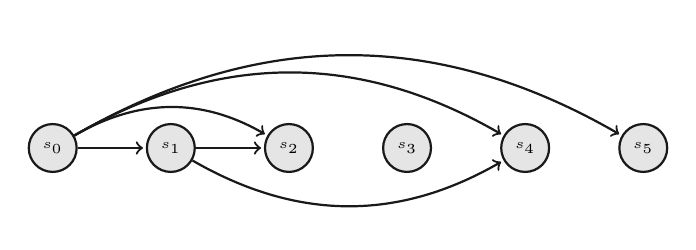
\begin{tikzpicture}[shorten >=1pt,->,scale=0.5]  
        \tikzstyle{sentence}=[circle,thick,draw=black!90,fill=black!10,minimum size=2mm]
		\tikzstyle{entity}=[circle,thick,draw=black!90,fill=black!10,minimum size=2mm]
        \tikzstyle{edge}=[draw=black!90, thick]

       \begin{scope}
       
         \node [sentence] (s0) at (0,0) {\tiny{$s_0$}};
         \node [sentence] (s1) at (3,0) {\tiny{$s_1$}};
         \node [sentence] (s2) at (6,0) {\tiny{$s_2$}}; 
         \node [sentence] (s3) at (9,0) {\tiny{$s_3$}}; 
         \node [sentence] (s4) at (12,0) {\tiny{$s_4$}};
         \node [sentence] (s5) at (15,0) {\tiny{$s_5$}}; 
 
 		\path[edge] (s0) edge [above] node[font=\tiny]{} (s1);
 		\path[edge, bend left = 30] (s0) edge [above] node[font=\tiny]{} (s2);
		\path[edge, bend left = 30] (s0) edge [above] node[font=\tiny]{} (s4);
 		\path[edge, bend left = 30] (s0) edge [above] node[font=\tiny]{} (s5);

 		\path[edge] (s1) edge [above] node[font=\tiny]{} (s2);
		\path[edge, bend right = 30] (s1) edge [above] node[font=\tiny]{} (s4);
           
        \end{scope}        
      \end{tikzpicture}

\\

\begin{tikzpicture}        
		 \node [] (n0) at (0,0) {};
         \node [] (label) at (0,0.8) {$P_W:$};
\end{tikzpicture}
 &
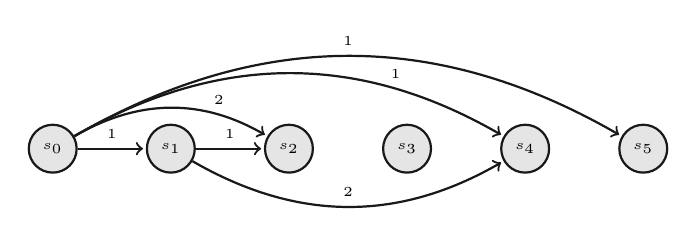
\begin{tikzpicture}[shorten >=1pt,->,scale=0.5]  
        \tikzstyle{sentence}=[circle,thick,draw=black!90,fill=black!10,minimum size=2mm]
		\tikzstyle{entity}=[circle,thick,draw=black!90,fill=black!10,minimum size=2mm]
        \tikzstyle{edge}=[draw=black!90, thick]

       \begin{scope}
       
         \node [sentence] (s0) at (0,0) {\tiny{$s_0$}};
         \node [sentence] (s1) at (3,0) {\tiny{$s_1$}};
         \node [sentence] (s2) at (6,0) {\tiny{$s_2$}}; 
         \node [sentence] (s3) at (9,0) {\tiny{$s_3$}}; 
         \node [sentence] (s4) at (12,0) {\tiny{$s_4$}};
         \node [sentence] (s5) at (15,0) {\tiny{$s_5$}}; 
 
 		\path[edge                ] (s0) edge [above, midway] node[font=\tiny]{$1$} (s1);
 		\path[edge, bend left = 30] (s0) edge [above, near end] node[font=\tiny]{$2$} (s2);
		\path[edge, bend left = 30] (s0) edge [above, near end] node[font=\tiny]{$1$} (s4);
 		\path[edge, bend left = 30] (s0) edge [above, midway] node[font=\tiny]{$1$} (s5);

 		\path[edge                 ] (s1) edge [above, midway] node[font=\tiny]{$1$} (s2);
		\path[edge, bend right = 30] (s1) edge [above, midway] node[font=\tiny]{$2$} (s4);
           
        \end{scope}        
      \end{tikzpicture}

\\

\begin{tikzpicture}        
		 \node [] (n0) at (0,0) {};
         \node [] (label) at (0,0.8) {$P_{Acc}:$};
\end{tikzpicture}
 &
   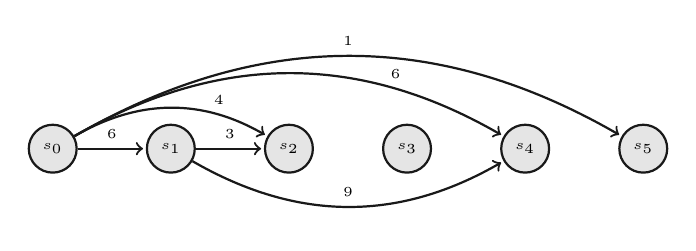
\begin{tikzpicture}[shorten >=1pt,->,scale=0.5]  
        \tikzstyle{sentence}=[circle,thick,draw=black!90,fill=black!10,minimum size=2mm]
		\tikzstyle{entity}=[circle,thick,draw=black!90,fill=black!10,minimum size=2mm]
        \tikzstyle{edge}=[draw=black!90, thick]

       \begin{scope}
       
         \node [sentence] (s0) at (0,0) {\tiny{$s_0$}};
         \node [sentence] (s1) at (3,0) {\tiny{$s_1$}};
         \node [sentence] (s2) at (6,0) {\tiny{$s_2$}}; 
         \node [sentence] (s3) at (9,0) {\tiny{$s_3$}}; 
         \node [sentence] (s4) at (12,0) {\tiny{$s_4$}};
         \node [sentence] (s5) at (15,0) {\tiny{$s_5$}}; 
 
 		\path[edge                ] (s0) edge [above, midway] node[font=\tiny]{$6$} (s1);
 		\path[edge, bend left = 30] (s0) edge [above, near end] node[font=\tiny]{$4$} (s2);
		\path[edge, bend left = 30] (s0) edge [above, near end] node[font=\tiny]{$6$} (s4);
 		\path[edge, bend left = 30] (s0) edge [above, midway] node[font=\tiny]{$1$} (s5);

 		\path[edge                 ] (s1) edge [above, midway] node[font=\tiny]{$3$} (s2);
		\path[edge, bend right = 30] (s1) edge [above, midway] node[font=\tiny]{$9$} (s4);
           
        \end{scope}        
      \end{tikzpicture}

\end{tabular}
\caption{$P_U$, $P_W$, and $P_{Acc}$ projection graphs.}

\label{fig:entity_projection}
\end{figure}


Distance between sentences can be integrated in the weight of the one-mode projection graphs to decrease the importance of links that exist between nonadjacent sentences. 
In this case, the weights of the projection graphs are divided by the number of sentences in between of two sentences. 

Inspired from the centrality measure in graph theory that measures the connectivity of nodes in a graph, the coherence of a text can be measured by computing the average outdegree of a projection graph as follow:

\begin{equation}
Coh(T) = AvgOutDeg(P) = \frac{1}{N} \sum_{\textit{i \ in 1..N}} outDegree(s_i),
\end{equation}
where $outdegree(s_i)$ is the sum of the weights associated to edges that leave $s_i$ and $N$ is the number of nodes in graph $P$. 

In our running example the average outdegrees in different projection graphs are as follows:

\begin{table}[!ht]
\centering
\begin{tabular}{l|l}
\hline
 $P$ & $ AvgOutDeg(P) = Coh(T)$ \\\hline
 $P_U$ & $\frac{1}{6} \left((1+1+1+1)+(1+1)+(0)+(0)+(0)+(0)) \right) = 1.00$ \\
 $P_W$ & $\frac{1}{6} \left((1+2+1+1)+(1+2)+(0)+(0)+(0)+(0)) \right) = 1.33$\\
 $P_{Acc}$ &$\frac{1}{6} \left((6+4+6+1)+(3+9)+(0)+(0)+(0)+(0)) \right) = 4.83$ \\
 $P_U\textit{, }Dist$ & $\frac{1}{6} \left((1+0.50+0.25+0.20)+(1+0.33)+(0)+(0)+(0)+(0)) \right) = 0.55$ \\
 $P_W\textit{, }Dist$ & $\frac{1}{6} \left((1+1+0.25+0.20)+(1+0.66)+(0)+(0)+(0)+(0)) \right)= 0.69$ \\
 $P_{Acc}\textit{, }Dist$ & $\frac{1}{6} \left((6+2+1.5+0.2)+(3+3)+(0)+(0)+(0)+(0)) \right)= 2.61$ \\ \\
 \hline
\end{tabular}
\end{table}

It is worth to mention that the proposed entity graph model by \newcite{guinaudeau13} is an unsupervised model meaning that the final average outdegree can be directly employed for comparing two texts with respect to their coherence. 
\newcite{guinaudeau13} assume that projection graphs of coherent texts contain more edges than the projection graph of incoherent texts. 
Therefore, the projection graph of coherent texts are expected to have higher average outdegree than the projection graph of incoherent texts.  


We see that for both entity graph and normalized entity graph models, using the syntactical information of entities do not improve the accuracy of these models. 
A reason for this is that by combining the weights of syntactical roles of the common entities between two sentences of an entity graph into the weight of the connecting edge between the sentences in $P_{Acc}$ the impact of the distance information is vanished.  
The presented example in Figure \ref{fig:pacc_vanishing_problem} illustrates this. 

\begin{figure}[!t]
\centering
\small
\begin{tabular}{@{}clclc@{}}
\hline
Projection & Sentence order &  Graph & Outdegree & Decision 
\\\hline
\multirow{2}{*}{$P_W$ }
&
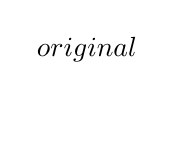
\begin{tikzpicture}        
		 \node [] (n0) at (0,0) {};
         \node [] (label) at (0,0.8) {$original$};
\end{tikzpicture}
&
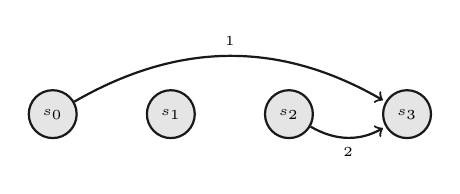
\begin{tikzpicture}[shorten >=1pt,->,scale=0.5]  
        \tikzstyle{sentence}=[circle,thick,draw=black!90,fill=black!10,minimum size=2mm]
		\tikzstyle{entity}=[circle,thick,draw=black!90,fill=black!10,minimum size=2mm]
        \tikzstyle{edge}=[draw=black!90, thick]

       \begin{scope}
       
         \node [sentence] (s0) at (0,0) {\tiny{$s_0$}};
         \node [sentence] (s1) at (3,0) {\tiny{$s_1$}};
         \node [sentence] (s2) at (6,0) {\tiny{$s_2$}}; 
         \node [sentence] (s3) at (9,0) {\tiny{$s_3$}}; 
 
 		\path[edge, bend left = 30] (s0) edge [above] node[font=\tiny]{$1$} (s3);
 		\path[edge, bend right = 30] (s2) edge [below] node[font=\tiny]{$2$} (s3);
           
        \end{scope}        
      \end{tikzpicture}

 &
 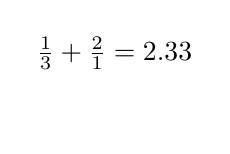
\begin{tikzpicture}        
		 \node [] (n0) at (0,0) {};
         \node [] (label) at (0,0.8) { $ \frac{1}{3} + \frac{2}{1}  = 2.33 $};
\end{tikzpicture}
&

\multirow{2}{*}{
\begin{tabular}{c}
$ 2.33 > 2 \Rightarrow $
\\
$correct$  
\end{tabular}
}
\\

&
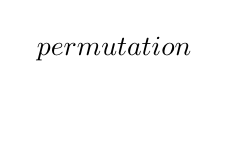
\begin{tikzpicture}        
		 \node [] (n0) at (0,0) {};
         \node [] (label) at (0,0.8) {$permutation$};
\end{tikzpicture}
&
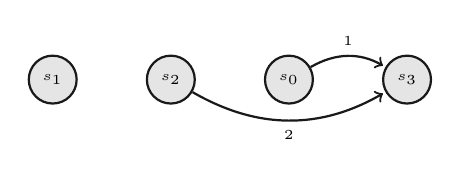
\begin{tikzpicture}[shorten >=1pt,->,scale=0.5]  
        \tikzstyle{sentence}=[circle,thick,draw=black!90,fill=black!10,minimum size=2mm]
		\tikzstyle{entity}=[circle,thick,draw=black!90,fill=black!10,minimum size=2mm]
        \tikzstyle{edge}=[draw=black!90, thick]

       \begin{scope}
       
         \node [sentence] (s1) at (0,0) {\tiny{$s_1$}};
         \node [sentence] (s2) at (3,0) {\tiny{$s_2$}};
         \node [sentence] (s0) at (6,0) {\tiny{$s_0$}}; 
         \node [sentence] (s3) at (9,0) {\tiny{$s_3$}}; 
 
 		\path[edge, bend left = 30] (s0) edge [above] node[font=\tiny]{$1$} (s3);
 		\path[edge, bend right = 30] (s2) edge [below] node[font=\tiny]{$2$} (s3);
           
        \end{scope}        
      \end{tikzpicture}

 &
 \begin{tikzpicture}        
		 \node [] (n0) at (0,0) {};
         \node [] (label) at (0,0.8) { $\frac{1}{1} + \frac{2}{2} =  2 $};
\end{tikzpicture}
&

\\ 
\hline
\\ 
\multirow{2}{*}{$P_{Acc}$ }
&

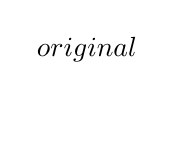
\begin{tikzpicture}        
		 \node [] (n0) at (0,0) {};
         \node [] (label) at (0,0.8) {$original$};
\end{tikzpicture}
&
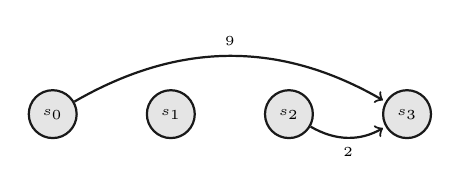
\begin{tikzpicture}[shorten >=1pt,->,scale=0.5]  
        \tikzstyle{sentence}=[circle,thick,draw=black!90,fill=black!10,minimum size=2mm]
		\tikzstyle{entity}=[circle,thick,draw=black!90,fill=black!10,minimum size=2mm]
        \tikzstyle{edge}=[draw=black!90, thick]

       \begin{scope}
       
         \node [sentence] (s0) at (0,0) {\tiny{$s_0$}};
         \node [sentence] (s1) at (3,0) {\tiny{$s_1$}};
         \node [sentence] (s2) at (6,0) {\tiny{$s_2$}}; 
         \node [sentence] (s3) at (9,0) {\tiny{$s_3$}}; 
 
 		\path[edge, bend left = 30] (s0) edge [above] node[font=\tiny]{$9$} (s3);
 		\path[edge, bend right = 30] (s2) edge [below] node[font=\tiny]{$2$} (s3);
           
        \end{scope}        
      \end{tikzpicture}

 &
 \begin{tikzpicture}        
		 \node [] (n0) at (0,0) {};
         \node [] (label) at (0,0.8) { $\frac{9}{3} + \frac{2}{1} = 5 $};
\end{tikzpicture}
&

\multirow{2}{*}{
\begin{tabular}{c}
$ 5 < 10 \Rightarrow $
\\
 $incorrect$
 \end{tabular}  
}
\\

&
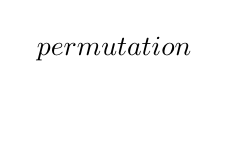
\begin{tikzpicture}        
		 \node [] (n0) at (0,0) {};
         \node [] (label) at (0,0.8) {$permutation$};
\end{tikzpicture}
&
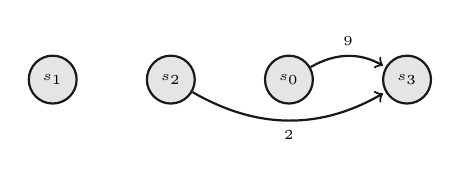
\begin{tikzpicture}[shorten >=1pt,->,scale=0.5]  
        \tikzstyle{sentence}=[circle,thick,draw=black!90,fill=black!10,minimum size=2mm]
		\tikzstyle{entity}=[circle,thick,draw=black!90,fill=black!10,minimum size=2mm]
        \tikzstyle{edge}=[draw=black!90, thick]

       \begin{scope}
       
         \node [sentence] (s1) at (0,0) {\tiny{$s_1$}};
         \node [sentence] (s2) at (3,0) {\tiny{$s_2$}};
         \node [sentence] (s0) at (6,0) {\tiny{$s_0$}}; 
         \node [sentence] (s3) at (9,0) {\tiny{$s_3$}}; 
 
 		\path[edge, bend left = 30] (s0) edge [above] node[font=\tiny]{$9$} (s3);
 		\path[edge, bend right = 30] (s2) edge [below] node[font=\tiny]{$2$} (s3);
           
        \end{scope}        
      \end{tikzpicture}

 &
 \begin{tikzpicture}        
		 \node [] (n0) at (0,0) {};
         \node [] (label) at (0,0.8) { $ \frac{9}{1} + \frac{2}{2} = 10 $};
\end{tikzpicture}
&
\\
\hline
\end{tabular}
\caption{An example of how syntactical roles vanish the effect of the distance information.}
\label{table:pacc_vanishing_problem}
\end{figure}

This example shows $P_W$ and $P_{Acc}$ of the same document. 
It is clear from the $P_W$ presentation of the original order of the document that in the entity graph representation of the document, sentence node $s_3$ shares respectively one and two entity nodes with sentence nodes $s_0$ and $s_2$. 
The weights of edges in $P_{Acc}$ representation of the original order depict that grammatical transition of the common entity between $s_0$ and $s_3$ is $S\ S$, because the weight of the edge between these two nodes is $9$ and $S$ is mapped to $3$. 
With the same reasoning, we can induce that the grammatical transitions of two common entities between $s_2$ and $s_3$ are $X\ X$. 
In Table \ref{table:pacc_vanishing_problem}, we compare the original outdegree of projection graphs that represent the original order of sentences and one of its permutations in that $s_0$ is removed from the original order and reinserted in the third position between $s_2$ and $s_3$. 
This example shows how the method of computing the weights of projection graphs influences the performance of the graph-based coherence model for the insertion task. 
As we discussed before an important factor in sentence ordering tasks is distance and 
 accumulating the associated numbers to the grammatical roles of entities discards the effect of distance. 



\subsubsection{Extensions}

\todo{citation}{Zhang et al. (ACL 2015)} use the semantic relations between named entities to not only cover the co-referential entities but also semantically related entities (e.g.\ Gates and Microsoft). 
They capture such semantic relations by leveraging world knowledge.
Both the \mbox{entity-graph} and \mbox{entity-grid} models improved by incorporating these relations. 
Analyzing the CoNLL 2012 dataset (Pradhan et al. 2013), they found that 42.34\% of the time, adjacent sentences do not share common entities. 
As a result methods that rely on strict entity matching would fail on these cases. 
average outdegree. 
The intuition behind the reachability score of nodes with outdegree zero is that this score reflects the tightness between this sentence the preceding part of the text. 
The reachability score is the sum of the weights from the first sentence node to the current sentence node. 
\todo{is it neccessary?}{Zhang et al. (ACL 2015) also explore a pattern so subgraphs within a window of three sentences, and use the frequencies of these distribution patterns over the entire document as additional features.} 
They combine these feature with the \mbox{entity-grid} model. 
They evaluate on sentence ordering and summary coherence rating. 
The main contribution of this paper is that incorporating world knowledge is beneficial for coherence modeling. 
They limit the semantic relation between entities to argument1-predicate-argument2, e.g., Gates-create-Microsoft.

 
\cite{petersen15} use several graph topology metrics to approximate different aspects of the discourse flow that can indicate coherence, such as the average clustering or betweenness of discourse entities in text. 
They investigate if graph properties, such as the clustering coefficient, or iterative graph ranking algorithms, such as PageRank,  can approximate document coherence. 
They conclude that the topological metrics that their employed to model the topology of graphs work on par with the average outdegree employed by  entity graph. 


\cite{dias15}  fill the grid in the entity grid with the occurrence of discursive information
(RST and/or CST \cite{?}(Castro Jorge et al. 2014)) such that an entry is one where an entity is part of a sentence that participate in a discursive relation.
Then define the bipartite graph as its original version ans use outdegree to measure coherence of texts. 
Their model outperforms the entity graph model for sentence ordering task on summaries produced by a multi-document summarizer. 
This may be justified by the availability of more CST relations than RST relations in multi-document summaries.
They argue that although the new information improve the results, obtaining discursive information is expensive. 


\cite{lioma16} eliminate the need for the projection graph with this intuition that projection incur significant loss of information present in bipartite graph.  
They present three new graph metrics that compute text coherence on the original bipartite graph. 
These metrics are obtained by different ways of normalizing the weights of the entity graph representation. 
That is different with our approach that normalize the weights of the projection graphs and uses outdegree as the final coherence score. 


\section{Lexical Approaches to Local Coherence}

Lexical chaining has been used in a number of applications such as news segmentation (Stokes, 2003), question-answering (Moldovan and Novischi, 2002), summarization (Barzilay and Elhadad, 1997), de- tection and correction of malapropisms (Hirst and St-Onge, 1995), topic detection (Hatch et al., 2000), topic tracking (Carthy and Sherwood-Smith, 2002), and keyword extraction (Ercan and Cicekli, 2007).

A text or discourse is not just a set of sentences, each on some random topic. 
Rather, the sentences and phrases of any sensible text will each tend to be about the same things -- that is, the text will have a quality of unity. 
This is the property of cohesion -- the sentences "stick together" to function as a whole. 
Cohesion is achieved through back-reference, conjunction, and semantic word relations. 
Cohesion is not a guarantee of unity in text but rather a device for creating it. 
As aptly stated by Halliday and Hasan (1976), it is a way of getting text to "hang together as a whole." Their work on cohesion has underscored its importance as an indicator of text unity.

Lexical cohesion is the cohesion that arises from semantic relationships between words. 
All that is required is that there be some recognizable relation between the words.
 
One of the basic approaches to lexical cohesion is \emph{Cohesion in English} \cite{halliday76}. 
Halliday and Hasan’s model of lexical cohesion is based on a division of the various lexical cohesive devices into two main categories: reiteration and collocation. 
Reiteration includes the repetition of the same word (mushroom – mushroom), the use of a synonym (sword – brand), the use of a superordinate (Jaguar – car), and the use of a general word (We all kept quiet. That seemed the best move.). 
All these devices have the function of reiterating the previous item, either in an identical or somewhat modified form, and this is the basis for the creation of a cohesive tie between the items.
Often the tie is strengthened by the fact that the items are co-referential, but as \newcite{halliday76} \textbf{Halliday and Hasan (1976: 282– 283)} note, this is not required for two items to be cohesive; even without co-referentiality, two occurrences of an item in a text will constitute a tie, as in the following example .

There’s a boy climbing that tree. Most boys do!

According to Halliday and Hasan, collocation is ``cohesion that is achieved through the association of lexical items that regularly co-occur'' (Halliday \& Hasan 1976: 284). 
This general definition of collocation may seem a little vague, but they do try to clarify it: the association is achieved when the lexical items have a tendency to appear in similar lexical environments or when they are related lexicosemantically. 
For example, boy and girl are cohesive because they have opposite meanings, but laugh and joke, and boat and row are also cohesive, although they are not systematically related, only ``typically associated with one another'' (Halliday \& Hasan 1976: 284–286).

What differentiates between collocation in the lexicographic sense, on the one hand, and in the cohesive sense, on the other, is the proximity of the items. In lexicography, collocation refers to adjacent items: the item investigated is called the node, and a restricted number of items (typically from four to six) positioned on either side of the node are its collocates. But since cohesion refers to connections between longer stretches of a text (clauses and sentences), items that are regarded as being related by collocation in the cohesive sense cannot be adjacent in that text. We can here reconsider Firth’s example of night and dark: if they occur next to each other, they are an instance of lexicographic col- location, but if they are separated by a longer stretch of text, their relationship ties together the clauses or the sentences in which they occur and they can be regarded as an instance of cohesive collocation.

Segmentation into a linear sequence of topically coherence segments generally assumes that the topic of a segment will differ from that of adjacent segments. It is also assumed that topic constrains lexical choice. either of all words of a segment or just its content words (i.e., excluding stop-words).
Topic relation is based on either semantic-relatedness or topic models. 
The elements for making connections are either sentences or a pseudo-sentences (i.e., fixed length string) whose relevant elements may be all the words or just content words .
All semantic-relatedness approaches to topic segmentation involve (1) a metric for assessing the semantic relatedness of terms withing proposed segments (2) a locality that specifies which units within a text are assessed for semantic relatedness, (3) a threshold for deciding how low relatedness can drop before it signals a shift to another segment.
Galley et al. (2003) use lexical chains to model lexical cohesion, rather than either word-stem frequencies or LSA-based concept frequencies.
Even though lexical chains exploit only term repetitions, rather than the wider range of relations. 
compactness of lexical chains captures locality of a topic. 
A similar approach is taken by Kan et al. (1998), though based on entity chains. 
This enables pronouns to be included as further evidence for intra-segmental semantic similarity. 

This type of relationship is the most problematic, especially from a knowledge representation point of view. Such collocation relationships exist between words that tend to occur in similar lexical environments. Words tend to occur in similar lexical environments because they describe things that tend to occur in similar situations or contexts in the world. Hence, context-specific examples such as {post office, service, stamps, pay, leave} are included in the class.

\newcite{morris91} models lexical cohesion by extracting all lexical chains. 
\begin{definition}
A sequence of related words is called \emph{lexical chain}. 
\end{definition}
A property of lexical chains is that they do not stop at sentence boundaries, and can connect words on a given span of text. 
Lexical cohesion provide a clue for the determination of coherence and discourse structure, and hence the larger meaning of the text \cite{morris91}. 


\newcite{stokes04} employ an auxiliary knowledge source, e.g.\ WordNet \cite{}, to extract lexical chains from texts. 
Their main intuition is that vocabulary in text segments with similar topics are mostly semantically related. 
Weak relations between words in lexical chains in a text is an indicator of topic shifts in the text. 

\newcite{benguosheng13} propose a bilingual lexical cohesion model for document-level machine translation.  
The coherence of the translated document is achieved by considering lexical cohesion items in the source document. 
The idea is that the strength of the semantic relation between two words should be retained in their counterparts in the translated document. 
In this way the translated document is easier to read if the source document is readable. 

\newcite{wongbillytm12} integrate lexical cohesion in assessment of translated documents. 
Lexical cohesion items in a translated document should be ideally similar to those in its associated human translation. 

\newcite{yannakoudakis12} measure coherence based on different features including the lexical relations between sentences. 
Instead of computing lexical chains, each sentence is represented by a vector of its words, and then the average of the cosine similarity between sentences encode how semantically they are related. 

\newcite{barzilay97} use WordNet to extract all lexical relations between words in a text in order to produce a coherent summary of the text.  

\newcite{somasundaran14} uses lexical chaining for measuring the quality of essays written by students. 
The main intuition is that the number of chains and their properties reveal quality of essays in terms of focus in topic and elaboration. 
Moreover, some extra features capture interactions between chains to model if the cohesive elements are organized in a coherent way. 
They employ different attributes of lexical chains in essays as coherence features. 


In a closely related study, \newcite{fenglijun09} use lexical chains to measure readability. 
Lexical chain features are employed to indicate the number of entities/concepts that a reader must keep in mind while reading a document.  

\newcite{flor13} present a coherence model based on lexical tightness among content words in a text. 
Lexical tightness represents the degree to which a text tends to use words that are highly inter-associated in a language. 
They show that lexical tightness strongly correlates with readability level of expertly rated reading materials. 

\newcite{foltz98} use Latent Semantic Analysis, which reflects second order co-occurrence associative relations, to characterize levels of lexical similarity for  for all possible pairs of sentences within paragraphs. 

Zhang et al. (ACL 2015) explain two major issues for retrieving world knowledge related to a document: 
\begin{itemize}
\item knowledge source: where can we obtain this knowledge? 
\item Knowledge selection: how do we pinpoint the most relevant ones?
\end{itemize}

In terms of knowledge source there are two type of sources: manually edited knowledge sources such as YAGO (Hoffart et al. 2013).
Yago consists of four million human-edited instances from on-line encyclopedias such as WikiPedia (Denoyer and Gallinari, 2007) and FreeBase (Bollacker et al., 2008).
The second category is automatically constructed knowledge bases which covers about 20 million instances extracted from row texts. 
Generally speaking, manually edited knowledge based have better accuracy but lower coverage, while automatically extracted knowledge bases are the opposite. 
The issue related to knowledge selection is that if to retrieve knowledge instances using exact or partial matching. 
The chance of exact matching of entities in a document with instances in knowledge base is low. 
In contrast, partial matching between arguments and entities usually increase coverage but the at risk of introducing more noise. 
Zhang et al. (ACL 2015) showed that reachability score of nodes in the projection graphs contributes more to coherence measurement than the 
Kunser et al. (JMLR 2015) use word embeddings to model the semantic relations between words of a document. 
The usage of word embeddings allow us to capture the distance or relative relatedness between individual words. 
Lijiwei and Hovy (EMNLP 2014) propose a deep neural coherence model based on distributed sentence representation. 
They limit coherence to ordering task that arrange a set of sentences in a coherent order. 
Word embedding approaches like \emph{word2vec}\ and \emph{GloVe}\ \cite{mikolov13c,pennington14} show that the semantic connection
between words can be captured by word vectors which are obtained by applying a neural network. 
The ability to train on very large data sets allows the model to learn complex relationships between words.


Somasudaran et al. (COLING 2014) hypothesize that attributes of lexical chains as well as interactions between lexical chains and explicit discourse elements, can harnessed for representing coherence. 
Coherence, the reader's ability to construct meaning from a document, is greatly influenced by the presence and organization of cohesive elements in the text (Halliday and Hasan, 1976; Moe, 1979). 
A lexical chain consists of a sequence of related words that contribute to the continuity of meaning based on word repetition, synonym and similarity. 
They build lexical chains and extract linguistically-motivated features from them. 
The number of chains and their properties, such as length, density and link strength, can potentially reveal discourse quality related to focus and elaboration. 
According to Morris and Hirst (1991), lexical cohesion is the result of chains of related words that contribute to the continuity of lexical meaning. 
Lexical chains tend to delineate portions of text that have a strong unity of meaning. 
They show that lexical chains can reveal different characteristic of discourse such as text unity, elaboration and detailing, variety, and organization. 


Coherent essays generally maintain focus over the main theme. 
Lexical chains presumably represent the main claim or position in persuasive texts, the main object or person in descriptive texts and the main story-line in narrative texts. 
Good writers usually initiate topics, ideas or claims and provide clear elaboration and reasons. 
That is, a sequence of many related words and phrases will be evoked to explain an idea provide an account of the writer's reasoning. 
While cohesiveness is vital for coherence, too much repetition of the same word can, in fact, harm the discourse quality (Witte and Faigley, 1981). 
Using a variety of words to express an idea or elaborate on a topic is generally a characteristic of skillful writing. 
In addition to cohesion, one other factor must be present for text to have coherence: organization (Moe, 1979; Prefetti and Lesgold, 1977). 
Thus it is important to organize ideas using clear discourse transitions.
Transitions from one topic to another, or from a topic to its subtopics, should be clearly cued in order to assist the reader's understanding of the discourse.
Consequently, in coherent writing, we would expect lexical chain patterns to synchronize with discourse cues that lead to topic continuity.  
In their work, nouns are the participants of lexical chains. 
Lin's thesaurus (Lin, 1998) is used to measure the similarity between nouns. 
They use a high threshold ($0.8$) to classify the relation between two words as the a strong relation, other relations are considered weak relations. 
Rus and Niraula (2012) find centered paragraph based on prominent syntactic roles. 
Milsakaki and Kukich (2000) use manually marked centering information and find that higher number of Rough shifts are indicative of lack of coherence. 
Wang, Harrington, and white (2012) combine the approaches from Barzilay and Lapata (2008), and Miltsakaki and Kukich (2000) to detect coherence breakdown points. 
The biggest difference between our model and Centering based models is that our model do not use syntactically prominent items or try to establish a center. Instead, multiple concurrent thematic chains can ``flow" through paragraphs and their features are used to model coherence. 
Our work also differs from systems using cohesion to measure writing quality (Witte and Faigley, a981; Flor et al., 2013), in that we focus on predicting the quality of discourse coherence. 


Higgins and Burstein (2007) use a Random Indexing model to model the similarity between sentences of an essay where sentences are represented via a vector. 
Their intuition is that related sentences in a text tend to use the same or similar words. While the use of similar terms does not guarantee relatedness, it is almost a precondition, and they believe that it should function well as a predictor of relatedness. 
The natural first candidate among vector-based approaches to semantics for use in assessing text coherence is the standard model of content vector analysis, used in information retrieval. 
In this model, each document is associated with a vector of the words in that document, and each word is represented as a vector listing the documents in which the word occurs. 
Latent Semantic Analysis (LSA) (Landauer and Dumais, 1997) is one of the old models in vector-space methods of semantic similarity using dimensionality reduction. 
LSA involves the application of Singular Value Decomposition to the document-by-term matrix in order to reduce its rank. 
Because information is lost in this compassion process, some similar vectors will be conflated, or moved closer whiting the space. 
LSA has proved to be a great improvement over the simple vector-space IR model for some domains. 
The term-term similarity scores it produces are more robust (Landauer et al., 1998, Haggins and Burstein (2007)).
LSA has been shown to be applicable to the task of establishing text coherence (Foltz et al. (1998)) although their application of LSA in this domain is very different from ours. 
There were some drawbacks with LSA models that do not exist in these days. 
For one thing, Singular Value Decomposition requires a numerical computation which is demanding both good possessing units and memory units. 
LSA is also very dependent on the corpus used to train it. 
Since term-occurrence within. documents is the basis for the generalizations it derives, it performs best when trained on corpora which are very topically coherent and which cover a diverse set of topics. 
An encyclopedia is a good text to use for LSA, but it is hard to obtain high quality encyclopedic texts as low cost, especially in large quantity. 
Random Indexing is more efficient method than LSA for term similarity. 
%% TO DO: what are some draw backs of LSA? why should we use word embeddings?

Higgins and Burstein (2007) also use a cutoff in similarity are taken to be related, while those below the cutoff are taken to be unrelated. 
Their model is basically a new cosine similarity model between word sentences. 


Kazantseva and Szpakowicz(COLING 2014) consider the problem of topic shift in a documents. 
They argue that on topical shifts in discourse are signaled by changes in vocabulary. 
They also assume that the type of referring expression, as extra information on lexical similarity, is an indicator of how accessible its antecedent is. 
The more accessible the antecedent likely to be and the more likely it is that the topic under has remained constant between the two mentions. 
They define a text-tilling model based on the cosine similarity over sentences. 
The segmenter explicitly measures the amount of lexical similarity between sentences, places where the similarity is low are likely to indicate a shift in topic. 
The idea that vocabulary shifts indicate topical shifts dates back to Youmans (1991). 
In scientific papers clarity is paramount, so the author will endeavor to state things explicitly and avoid ambiguity. 
The less complicated the document, the less it is to explicitly repeat terminology. 
In contrast, in literature, word repetition is not only uncommon, but it is usually a sign of bad writing.  
Hears (1994,1997) describes TextTiling, an algorithm which identifies topical shifts by sliding a window through a document and measures the cosine similarity between adjacent windows. 
The drop in similarity measures signals shifts of topics. 
Marathe (2010) used lexical chains such that the beginning and the end of a lexical chain tend to correspond to the beginning and the end of the a topically cohesive segment.
Lexical resources, such as ontologies and knowledge bases may help to improve the quality of segmentations, but such resources are not always available. 
They also may cause problems with precision. 
MCSeg is one of the segmenters based on the cosine similarity between sentences that is developed by Malioutov and Barzilay, 2006. 



\section{Coherence in Applications}
\label{sec:rel-coh-applications}

Discourse structure plays a crucial role in different applications such as summarization, information extraction, essay analysis and scoring  \cite{burstein10}, 
sentiment analysis, and assessing the naturalness and coherence of automatically generated texts. 
In this section, we review different tasks employed for evaluating coherence models. 
We then explain why among these models, we choose readability assessment and text summarization for our evaluation purpose in this thesis. 
 
In order to evaluate a coherence model, a scoring function is required \cite{karamanis04}.   
A scoring function is a function that returns a score (or a set of scores) for the coherence of a text.  
This function is an increasing function; it returns higher scores for more coherent texts. 

\textbf{OVERLAP WITH EVALUATION IN COHERENCE FORMULATION}
Early work, which are inspired by Centering Theory, define different coherence functions based on the constraints introduced by Centering.    
For instance,  \newcite{poesio04, miltsakaku00}, as one of the informal Centering-based coherence scoring functions, propose a scoring function based on the number of each transition type in a text.  
The function returns higher scores for texts that have many number of CONTINUE transitions and less number of SHIFT transitions. 
This scoring function cannot be utilized by text generation systems \cite{karamanis04}. [WHY?] 
\newcite{cheng02} present a genetic algorithm which handles the interaction between sentences.  
The scoring function uses the entity-based relations among sentences with features weighted according to preferences in Centering Theory.  
\newcite{kibble00} propose as scoring function based on the count the number of CT-based violations in texts. Texts with lower number of violations are more coherent. 

As it has been shown, CT is open-ended enough for one to propose new metrics which appear to be as plausible a some existing ones from a purely theoretical point of view. 
\newcite{karamanis04} explain that it is practically impossible to come up with an experimental design which accounts for the predictions of all aspects of coherence metrics at the same time. 

The entity grid coherence model \cite{barzilay05a} is evaluated on three tasks: sentence ordering, summary rating and readability assessment. 
In these tasks, coherence is taken as a relative property, rather than binary, of texts: Given a pairs of texts, which one is more coherent? 
They use a parametric scoring function based on the coherence features extracted from entity grid representations of texts.
Parameters of this function is trained by a machine learning approach, such that the function best fits to the evaluation task and data. 
Therefore, the evaluation task should be designed in a way to model coherence difference between texts. 
Following \cite{barzilay05a}, other models \cite{} also use three tasks: sentence ordering, summary rating, and readability assessment. 



\subsubsection{Sentence Ordering}
It is known that the order of information in coherent texts is such that they are easy to follow \cite{lapata03,barzilay04,karamanis04b,barzilay05a,soricut06}. 
As it is explained in the definition of coherence, a text is more than a random concatenation of sentences; so the order of sentences affects how difficult the presented information in a text can be understood.  
Given the above fact, a document can be taken as an unordered bag of sentences and the task would be to find the ordering of the sentences that maximizes coherence according to a model. 
Unfortunately, finding the best ordering is NP-complete \cite{?} and non-approximable \cite{althaus04}.
Therefore, this task need to be simplified to be used for coherence evaluation. 
Two restricted versions of the sentence ordering tasks are the discrimination task, and the insertion task. 
In both subtasks the model is examined to see whether it is able to distinguish between the correct (original) order of sentences in a document and an incorrect (non-original) one. 

\paragraph{Discrimination.}
The discrimination task is based on this fact that the original order of sentences in a document is taken as the best order and any scrambling of sentences disturbs the perceived coherence of the document. 
By rearranging the order of sentences of a document, the document becomes more difficult to understand or less coherent, because the order of presented information is disturbed. 

More formally, let $COH_M(d)$ be the coherence estimation of document $d$ by the coherence model $M$ and $p$ be a version of $d$ that its sentences are randomly permuted, then the coherence model $M$ should ideally distinguish document $d$ a more coherent document than $p$:

\begin{equation}
COH_M(d) > COH_M(p). 
\end{equation}
where $COH_M$ is the scoring function defined by model $M$. 
\newcite{barzilay08} assume that the $COH_M(d)$ is a linear function of coherence features, which are defined as the entity transitions in the entity grid model, as follows:

\begin{equation}
COH_M(d) = \vec{w}^{T}.\vec{t}
\end{equation}
%
where $w$ is a vector of parameters, i.e.\ weights, and $t$ is the feature vector representing the coherence of $d$. 
The goal of the learning procedure is learn the best values for parameters $w$ in order to minimize the number of violations of pairwise rankings provided in the training set. 
The learning problem typically treated as a Support Vector Machine (SVM) constraint optimization problem, and can be solved using the search technique implemented in $SVM_{ligh}$\footnote{link to the package} \cite{joachims02} package. 

A model assigns local coherence values with the original document and its permutation, if the score for the original order of sentences of a document is higher than the score of the permutation version of sentence then the output of our system being considered correct. 
Because the relative quality of different permutations is unknown, the dataset includes only pairwise rankings that comprise the original document and one of its permutations.

Two evaluation metrics seem suitable for this task: accuracy and F-measure. 
Accuracy measures how correctly a coherence model discriminates the original order of a document from its different permutations.
It equals the number of times the model assigns a higher score to the original document than the score that it gives to a permutation, divided by the number of comparisons.

\begin{equation}
Acc  = \frac{\#\textit{ of correct predictions}}{\#\textit{ of comparisons}}
\end{equation}

F-measure is also frequently used for this task, because the model may assigns the same score to a permutation and the original document. 
In order to compute F-measure, we need to compute recall and precision as follow:

\begin{equation}
recall = \frac{correct}{total},
\end{equation}
where $total$ is the total number of test samples no matter if on them the model can make a decision or not. 

\begin{equation}
precision = \frac{correct}{decisions},
\end{equation}
where $decision$ is the number of samples on that the model made a decision.

\begin{equation}
F1 = 2.\frac{precision \cdot recal}{precision + recall}
\end{equation}

The obtained performance by different coherence models \cite{} on the discrimination task is a reasonable. 
It is mainly because the discrimination task can be easily solved without any notions of coherence. 
Discrimination specially becomes easier for longer documents, since the average random permutation grows less similar to the original document. 
The insertion task, the second related task to sentence ordering, somewhat overcomes this easiness. 


\subsubsection{Insertion}

The insertion task \cite{chenerdong07}, similar to the discrimination task, is designed to evaluate the ability of a coherence model in distinguishing the proper order of sentences in a document from the other orders. 
The permutation task is easy to be solved, especially for documents with many sentences, because  permuting whole sentences yields a version of document that is very different, and therefore easier to distinguish, from the original document. 
The insertion task provide permutations that are not very different with original version of documents. 

The intuition behind the insertion task is that given a document where one of its sentences is removed, the perceived coherence of the document is discarded, because a gap is created between sentences. 
The removed sentence can be inserted in between of any two sentences in the document and creates a permutation of the original document.  
A coherence model should ideally assign a higher coherence score to a permutation in which the removed sentence is located in its original position. 

Given a document with $n$ sentences, if the sentence at position $i$ is removed then there are $n$ possible positions, including the position $i$, to reinsert this sentence and create a permutation of this document. 
Table \ref{table:insertion_task} shows an example of removing the sentence in position $0$ ($\underline{A}$) of a document with four sentences, $\left \{ A, B, C, D \right \}$, and reinserting the sentence in all possible positions. 
 

\begin{table}[!ht]
\centering
\begin{small}
\begin{tabular}{cc|cccc}
position & original document  & \multicolumn{4}{c}{permutations}\\
\hline
$0$ & $\underline{A}$ & $\underline{A}$ & $B$ & $B$ & $B$\\
$1$ & $B$ 			  & $B$  & $\underline{A}$ & $C$ & $C$\\
$2$ & $C$			  & $C$ & $C$ & $\underline{A}$ & $D$\\
$3$ & $D$			  & $D$ & $D$ & $D$ & $\underline{A}$\\
\end{tabular}
\end{small}
\caption{}
\label{table:insertion_task}  
\end{table}

Two evaluation metrics are employed for this task: accuracy and the insertion score (Ins.). 
Accuracy measures for how many sentences, out of the all sentences of a document, a coherence model exactly predicts the original position of the sentence as the best point to reinsert it. 
Therefore the accuracy is computed as follows:

\begin{equation}
Acc = \frac{1}{D}\sum_{d \in D}\frac{\#\textit{ of correctly placed sentences in d}}{\#\textit{ of sentences in d}}
\end{equation}
%
where $D$ is the set of documents in a dataset.  
By averaging over documents, longer documents do not dis-proportionally influence the results. 

In complement to accuracy, the insertion score is also introduced by \newcite{elsner11b} for evaluation. 
This score  –-- the higher, the better –--  is a positional score that measures how far the predicted position of a sentence by a coherence model is from the original position of the sentence. 
For each document this score is normalized by the length of document to be unbiased to the number of sentences in a document. 

More formally, this score is computed as follows:
\begin{equation}
Ins. = 1 - \frac{o - p}{norm(N, p)},
\end{equation}


\begin{equation}
norm(N, p) = \frac{1}{2*N} (p * (p-1) + (N - p + 1)*(N - p)),
\end{equation}
where $o$ and $p$ are respectively the original position of a removed sentence and its proposed position by the model. 
$N$ is the number of sentences in a document.  


Besides practical applications, insertion has three properties that make it well-suited for evaluation of coherence models. 
First, a document with $n$ sentences can be evaluated exactly in $n^2$ time, which, though it can be significant, is still much faster than ordering and does not involve a potentially error-prone search.
Second, it is very difficult for documents with many sentences to solve this task, because permutations only differ by one sentence.  
Third, in comparison with the permutation task, a document is compared to many more permutations. 
The system output is considered correct if the document associated with the highest local coherence score is the one in which the sentence is reinserted in the correct position. 

Sentence ordering task do not measure all aspects of coherence. 
Admittedly, the synthetic data used in the ordering tasks partially approximate coherence violations that human readers encounter in machine generated texts. 


\subsubsection{Readability Assessment}

Assessing the degree of readability of a text has been a field of research as early as the 1920's. Dale and Chall define readability as “the sum total (including all the interactions) of all those elements within a given piece of printed material that affect the success a group of readers have with it. The success is the extent to which they understand it, read it at optimal speed, and find it interesting” (Dale and Chall, 1949). It has long been acknowledged that readability is a function of text characteristics, but also of the readers themselves. The literacy skills of the readers, their motivations, background knowledge, and other internal characteristics play an important role in determining whether a text is readable for a particular group of people. 

Many readability metrics have been established as a function of shallow features of texts, such as the number of syllables per word and number of words per sentence (Flesch, 1948; McLaughlin, 1969; Kincaid et al., 1975). These so-called tra- ditional readability metrics are still used today in many settings and domains, in part because they are very easy to compute. Their results, however, are not always representative of the complexity of a text (Davison and Kantor, 1982). They can easily misrepresent the complexity of technical texts, or reveal themselves un-adapted to a set of readers with particular reading difficulties. Other formulas rely on lexical information; e.g., the New Dale-Chall readability formula consults a static, manually-built list of “easy” words to determine whether a text contains unfamiliar words (Chall and Dale, 1995).

Researchers in computational linguistics have investigated the use of statistical language mod- els (unigram in particular) to capture the range of vocabulary from one grade level to another (Si and Callan, 2001; Collins-Thompson and Callan, 2004). These metrics predicted readability better than traditional formulas when tested against a corpus of web pages. The use of syntactic fea- tures was also investigated (Schwarm and Osten- dorf, 2005; Heilman et al., 2007; Petersen and Ostendorf, 2009) in the assessment of text reada- bility for English as a Second Language readers. While lexical features alone outperform syntactic features in classifying texts according to their reading levels, combining the lexical and syntac- tic features yields the best results.
Several elegant metrics that focus solely on the syntax of a text have also been developed. The Yngve (1960) measure, for instance, focuses on the depth of embedding of nodes in the parse tree; others use the ratio of terminal to non- terminal nodes in the parse tree of a sentence (Miller and Chomsky, 1963; Frazier, 1985). These metrics have been used to analyze the writing of potential Alzheimer's patients to detect mild cognitive impairments (Roark, Mitchell, and Hollingshead, 2007), thereby indicating that cognitively motivated features of text are valua- ble when creating tools for specific populations. 


Coherence is a about relations between sentences that make a text different with an unrelated collection of sentences. 
It is a crucial factor in text quality assessment systems such as readability assessment and essay scoring systems.  
Sentences in well-written texts are semantically related such that the interpretation of  relations is easy to understand for readers.  

Coherence is very important for automatic text generation systems, since the output text is supposed to be readable. 
For example, an automatic text summarization system produces a gist of information presented in its input document(s) in an interpretable way. 
The other example is machine translation systems where a document in a language --- known as the source language --- is translated in another language --- known as the target language. 
If machine translation models do not take coherence into account then output document is not readable in the target language.   

Readability describes how easily a document can be read and understood. 
Some research papers \cite{} estimate the difficulty of a document by means of the time with that a reader can process and understand the document. 
Indeed, the difficulty of a document for its readers is beyond the surface aspects of the document such as employed vocabularies, the length of sentences, and etc. 
Discourse level factors of a document (e.g. coherence) plays a critical role in overall understanding of the document. 
Sentences of more coherent documents are supposed to be connected so that sentences become less ambiguous and information flow smoothly through the document. 

The task of readability assessment aims to distinguish texts which are difficult to read from texts which are easier to read. 
\newcite{guinaudeau13} treat the readability assessment task as a ranking task: Given a pair of document which one is easier to read. 

As before,  evaluate coherence models can be evlauted using accuracy and F-measure metrics. 
The accuracy measures how often a coherence model correctly distinguishes the version of an article from Encyclopedia Britannica more difficult than its version from Britannica Elementary. 
F-measure is also computed based on the precision and recall as explained in previous experiments. 

Higgins et al. ("Evaluating multiple aspects of coherence in student essays") evaluate multiple aspects of coherence in essays by defining some features based on semantic similarity measures and discourse structures. 
Some features include the relatedness between the essay and the topic and some other capture the relatedness between discourse elements (e.g. intra-sentential quality and sentence-relatedness within discourse segments. 
In earlier work, Folz et al. (1998) and Wiemer-Hastings and Graesser (2000) have developed coherence aspects of student writing.
Their system measures lexical relatedness between text segments by using vector-based similarity between adjacent sentences.
This linear approach to similarity scoring is in line with the TextTiling scheme (Hearst and Plaunt, 1993; Hearst 1997), which may be used to identify the subtopic structure of student essays. 
Miltsakaki and Kukich (2000) have also addressed the issue of establishing coherence of student essays, using the Rough shift element of Centering Theory. 
Higgins et al. () adopted a vector-based method of semantic representation: Random Indexing (Kanerva et al. 2000; Sahlgren, 2001) while other work use Latent Semantic Analysis as a semantic similarity measure. 
Their output shows that the semantic similarity between sentences is not as promising as other features. 
It relatively is rare to find a sentence which is not related to anything in the same discourse. 

\newcite{beigman13} use the lexical relations between words of a text to model the quality of the text. 
Their model is inspired by this fact that a text segmentation algorithm which uses information about patterns of word co-occurrences can detect sub-topic shifts in a text (Riedl and Biemann, 2012; Misra et al., 2009; Eisenstein and Barzilay, 2008) indicates that texts contain some proportion of more highly associated word pairs (those in subsequent sentences within the same topical unit) and of less highly associated pairs (those in sentences from different topical units). 
They illustrate the patterns of the distribution of semantically related words correlate with the writing quality. 
Their scoring function is obtained by binning the distribution of point wise mutual information, PMI, of any word pairs. 
Texts with many word pairs that have high PMI are more coherent than texts whose word pairs have small PMI. 
They evaluate their model to rank student essays with respect to their readabilities. 


\newcite{burstein10} use the same scoring function that is used by \newcite{barzilay05}. 
They also use F-measure for evaluation. 
The main contrinution of this paper is that they collect some some essay data and ask human annotators to read it and classify them into two category low- and high- coherence. 

\newcite{thompson04} approaches readability assessment as a classification task over grad level for texts. They do not explicitly use any coherence model, but use a language model. 

\newcite{kate10} consider the readability assessment task as a regression task. 
Their system is trained using diverse features based on syntax and language models which are generally indicative of readability. 
They collect a readability dataset consisting of texts in different genres. 
The text  is judged for its readability by six to ten human annotators who assign each text a rating on a 5-point scale to indicate how readable the text is where readability is defined as a subjective judgement of how easily a reader can extract the information that writer intended to convey. 
They compute the Pearson correlation between values of different features and the average human ratings associated with documents to measure which feature is more informative for this task. 
Although they do not use any coherence feature in their experiments but their results show that discourse features such as language model features are strongly correlated with human ratings. 

\subsubsection{Text Summarization}
The summary coherence ranking task is based on this intuition that a coherence model that exhibits a high agreement with human judges accurately captures the coherence properties of the machine generated texts. 
In this task, we test the ability of our coherence models to assess coherence by comparing rankings induced by a model against rankings elicited by human judges. 
Moreover, this task more close to real application of coherence in automatic text summarization.

\newcite{barzilay08, mesgar14} use a summarization dataset to evaluate their coherence models (i.e., the entity grid model and the entity graph models).  
The dataset contains $80$ pairs of summaries extracted from Document Understanding Corpus (DUC) $2003$. 
The corpus used in DUC 2003 includes multi-document summaries generated by human writers and by automatic summarization systems. 
In order to learn a ranking, we require a set of summaries, each of which has been rated in terms of coherence. 
This ratings are not provided by DUC summary evaluators. 
In DUC $2003$, the quality of system generated summaries was assessed with respect to several factors ranging from grammar, to content selection, fluency, and readability. 
Coherence was indirectly evaluated by noting the number of sentences indicating an awkward time sequence, suggesting a difficult to interpret relationship between sentences, or being semantically incongruent with their other sentences. 
\newcite{barzilay08} obtained judgments for automatically generated summaries from human subjects\footnote{\url{http://homepages.inf.ed.ac.uk/mlap/coherence/}}.
They randomly selected $16$ input documents and five systems that had produced summaries for these documents, plus the reference summaries written by humans. 
Coherence ratings were collected during an elicitation study by $177$ unpaid volunteers, all native English speakers. 
Participants first saw a set of instructions that explained the task, and defined the notion of coherence using multiple examples. 
The summaries were randomized in lists following a Latin square design ensuring that no two summaries in a given list were generated from the same document cluster. 
Participants were asked to use a seven-point-scale to rate how coherent the summaries were without having seen the source texts. 
The ratings (approximately $23$ per summary) given by our subjects were averaged to provide a rating between $1$ and $7$ for each summary. 
In order to to validate the quality of the annotations of how well humans agree in their coherence assessment, several tests have been done such as leave-one-out re-sampling, by correlating the data obtained from each participant with the mean coherence ratings obtained from all other participants. 
The inter-subject agreement was $r = 0.768$ ($p < 0.01$). 
In another annotation qualification test, they examined the effect of different types of summaries (human- vs. machine-generated.) concluding that human summaries are perceived as significantly more coherent than system-generated ones. 
The set of training materials contained $6 × 16$ summaries (average length $4.8$), yielding $c(6,2) × 16 = 240$ pairwise rankings. 
Because human summaries often have identical (high) scores, pairs of such summaries from the training set have been eliminated. 
Consequently, the resulting training corpus consisted of $144$ summaries. 
In a similar fashion, $80$ pairwise rankings for the test set have been obtained. 
Human coherence scores are associated with each pair of summarized documents \cite{barzilay08} Each of pair of the test set is being composed by two summaries of a same document where the score of one of the summaries is significantly higher than the score of the second one. 
Even though all summaries are of approximately the same length ($114.2$ words on average), their sentence length can vary considerably. 
Indeed, more coherent summaries tend to have more sentences and contain less entities

Considering this setting, Summary coherence rating can be also formulated as a ranking learning task.
Given a pair of summaries, one more coherent than the other, the objective of the task is to order the two summaries according to local coherence.

For evaluation purposes, similar to the discrimination  in the sentence ordering task, we use  accuracy and F-measure where the former corresponds to the number of correct ranking divided by the number of comparisons, and the latter the average of recall and precision measures.

Summarization based on the discourse structure relies on the connectivity style of elements of input text. 
Elements of text that loosely connect to other elements of the text can be omitted from a discourse without diminishing its readability or altering its content. 
Information on the discourse relations that link specific segments was used to distinguish material that should or should not be included in summaries. 
The information on discourse configuration is a good indicator for which segments should show up in the summary (Louis et al. 2010). 
This approach instantiates a set of design of choices for approaches to summarization on the basis of discourse structure.

First, it is an instance of extractive summarization, which selects the most prominent sentences for a summary.
This contrasts with sentence compression, which shortens the individual sentences. 
A second design choice involves the goal of the summary: Daume III and Marcu (2002) attempt to derive informative summaries that. represent the textual content of documents. 
An alternative goal, useful in summarizing scientific articles, involves highlighting the contribution of an article and relating it to previous work. 
With indicative summaries, the goal is to facilitate the selection of documents that are worth reading (Barzilay and Elhadad, 1997). 
A third design choice involves assumptions about the document to be summarized.
While  Daume III and Marcu (2002) assume a hierarchic structure, other approaches just take it to be flat. 
For example in summarizing the scientific papers, Teufel and Moens (2002) assume that a paper is divided into research goal (aim), outline of the paper (textual), presentation of the paper's contribution (methods, results, and discussion), and presentation of other work (other). 
They classify individual sentences for membership in these classes by discourse segmentation. 
This strategy is especially fruitful if the summarization concentrates on specific core parts of a document rather than on the document as a whole. 
Teufel and Moens (2002) do not assume that all sentences within a given section of the paper belongs to the same class, but they do find that adherence to a given ordering differs by scientific field: Articles in the natural sciences appear more sequential in this respect than the Computational Linguistics articles that they are targeting. 
A fourth design decision involves the type of document to be summarized.
Most summarization work targets either news or scientific articles. 
This choice has wide ramification for a summarizer because the structure of these documents is radically different. 
 
The ``inverted pyramid" structure of news articles means that their first sentences are often good summaries, while for scientific articles, core sentences are more evenly distributed. 
This difference shows, for instance in the evaluation of Marcus's (2000) summarizer, which was developed on the basis of essays and argumentative text.
A final design choice involves the way a summarizer identifies the discourse structure on which their summarization is based. 
While Marcu (2000) crucially relies on cue phrases and punctuation for identification of elementary and larger discourse units. 
Teufel and Moens (2002) characterize discourse elements by features like location in the document, length, and lexical and phrasal cue elements and citations. 
The third method uses the lexical chains that can be used for both extractive and compression (abstractive): For Barzilay and Elhadad (1997), important sentences comprise the first representative element of a strong lexical chain and it is these sentences that are selected for the summary. 
The use of lexical chains allows topicality to be taken into account to heighten the quality of summaries. 

Clarke and Lapata (2010) require the entity that serves as the center of a sentence (in the sentence of the Centering Theory) be retained in a summary. 
Schilder (2002) shows that discourse segments with low topicality should occupy a low position in a hierarchical discourse structure that can be set for extractive summarization. 
Barzilay and Lapata (2008) were the first researchers to recognize the potential value of entity chains and their properties for assessing text quality. 
They showed how one could learn patterns of entity distribution from a corpus and then use the patterns to rank the output of the statistical generation. 
Inspired by Centering Theory  (Grosz, Joshi and Weinstein 1995) Barzilay and Lapata (2008) consider patterns of local entity transitions. 
A local entity transition is a sequence ${s,o,x,-}^n$ that represents entity occurrences and their syntactic roles in n successive sentences. 
Since each transition has a certain probability in a given grid, each text can be viewed as a distribution over local entity transitions. 
A set of coherent texts can thus be taken as a source of patterns for assessing the coherence of new texts. 
Coherence constrains are also modeled in the grid representation implicitly by entity transition sequences, which are encoded using a feature vector notation: each grid $x_{ij}$ for document $d_i$ is represented by a feature vector:
$ \phi(x_{ij}) = (p_1(x_{ij}),p_2(x_{ij}),...,p_m(x_{ij}))$
where $m$ is the number of predefined entity transitions. 
To evaluate the contribution of three types of linguistic knowledge to model performance (i.e., syntax, coreference resolution, and salience). Barzilay and Lapata (2008) compared their model to models using linguistically impoverished representations. 
Omitting syntactic information is shown to cause a uniform drop in performance, which confirms its importance for coherence analysis. 
Accurate identification of correferring entities is a prerequisite to the derivation of accurate salience models and salience has been shown to have a clear advantage over other methods. 
Thus, Barzilay and Lapata provide empirical support for the idea that coherent texts are characterized by transitions with particular properties that do not hold for all discourse. 
In this work, a sentence is a bag of entities associated with syntactic roles. 
A mention of an entity, though may contain more information than just its head and syntactic role. 
Thus, Elsner and Charniak (2008a) inspired by work on coreference resolution, consider additional discourse-related information in referring expressions - information distinguishing between familiar entities from unfamiliar ones and salient entities from non-salient ones.   

% As before, significance is tested with the Student’s t-test accounting for the Bonferroni correction.


% \begin{table}[!t]
% \centering
% \begin{small}
% \begin{tabular}{l|cc@{}l}
%  & Acc. & F  &\\\hline
%  B\&L & $0.833$ &  &\\\hline

%  & \multicolumn{3}{|c}{Entity graph, G\&S} \\\hline 
% $P_U$ & $0.800$ & $0.815$ &  \\
% $P_W$ & $0.613$ & $0.613$&* \\
% $P_{Acc}$ & $0.700$ & $0.704$& \\  
% $P_U$, \textit{Dist} & $0.650$ & $0.658$ \\
% $P_W$, \textit{Dist} & $0.525$ & $0.525$  \\
% $P_{Acc}$, \textit{Dist} & $0.700$ & $0.700$  \\
% \hline 

%  & \multicolumn{3}{|c}{Normalized entity graph} \\\hline 
% $P_U$ & $\textbf{0.800}$ & $\textbf{0.815}$&  \\
% $P_W$ & $0.775$ & $0.775$& \\
% $P_{Acc}$ & $0.788$ & $0.788$& \\  
% $P_U$, \textit{Dist} & $0.650$ & $0.658$ \\
% $P_W$, \textit{Dist} & $0.738$ & $0.738$  \\
% $P_{Acc}$, \textit{Dist} & $0.750$ & $0.750$  \\
% \end{tabular}
% \end{small}
% \caption{Summary Coherence Rating, B\&L and entity
%   graph vs.\ normalized entity graph}
%  \label{table:summary_coherence_ranking}
% \end{table}
% %%%%%%%%%%

% Table \ref{table:summary_coherence_ranking} displays reported results of $B\&L$ and reproduced results of the entity graph and our normalized entity graph. 
% Unlike the sentence ordering task, accounting for the distance information between two sentence nodes (\textit{Dist}) tends to decrease the performance of graph models. 
% This difference is explained by the fact that a human summary, which is usually considered more coherent by humans judges, is inclined to contain more (and shorter) sentences than a summary generated by machines. 
% As adding distance information diminishes the value of our local coherence score (i.e. outdegree), distinguishing between the coherence and incoherent summaries becomes more difficult. 
% Therefore, both graph-based models obtain better results without incorporating the distance information. 

% Moreover, in contrast to the sentence ordering experiment, when we employ the number of entities ``shared” by two sentences as weights of projection graphs ($P_W$), models obtain lower values of accuracy and F-measure, than $P_U$. 
% This behavior could be because the number of sentences contained in the less coherent summaries. 
% Summaries generated by machines contain a smaller number of sentences where each sentence contains more entities on average. 
% This means that, in these summaries, two sentences are more likely to share a larger number of entities and therefore have a
% higher local coherence score when the $P_W$ projection graph is used.  
% The $P_{Acc}$ in the entity graph models obtains slightly better accuracy and F-measure than $P_W$. 


% Normalizing significantly improves the results of $P_W$  and $P_{Acc}$. 
% With the same reason to the entity graph model, distance information degrades the results for the normalization graph too. 
% $P_U$ is still slightly better than both $P_W$ and $P_{Acc}$, but in contrast to the entity graph, this difference is not statistically significant showing an advantage of our normalization method. 
% In the entity graph model, three projection graphs are proposed and as Table \ref{table:summary_coherence_ranking} shows their results are statistically different. 
% Our normalization method makes the difference between the results negligible. 
% So in production, there would be no difference between different projection graphs if the normalization method is used. 




% We use the readability dataset collected\footnote{\url{http://homepages.inf.ed.ac.uk/ mlap/coherence/.}} by \newcite{barzilay03b}, and used by \newcite{barzilay08,guinaudeau13}, from the Encyclopedia Britannica and Britannica Elementary. 
% The former contain the original and full articles and the latter version is targeted at children. 
% The dataset contains $107$ articles from the full version of the Encyclopedia Britannica and their corresponding simplified articles from Britannica Elementary ($107 + 107 = 214$ articles in total).
% Although these texts are not explicitly annotated with readability levels, they still represent two broad readability categories, namely, difficult and easy. 
% The collected articles of Encyclopedia Britannica are longer than their corresponding articles of Britannica Elementary in terms of number of sentences ($83.1$ sentences vs $36.6$ on average). 


% In order to estimate the complexity of a text, the graph-based coherence models compute the local coherence score for each text in the two categories.  
% Texts associated with the higher score is considered to be the more readable as it is more coherent, needing less interpretation from the reader than a text associated with a lower local coherence score. 


% We compare graph-based coherence models (i.e., the entity graph model and the normalized entity graph model) with the entity grid model (B\&L) as a coherence model, (S\&O) as a readability assessment model, and (B\&L $+$ S\&O) that is taken as an enriched readability assessment model with proposed coherence features in B\&L. 


% Table \ref{table:bri_ele} summaries the results of these models. 

% \begin{table}[!t]
% \centering
% \begin{small}
% \begin{tabular}{l|cc@{}l} 
%   & Acc. & F  &\\\hline
%   S\&O & $0.786$ & &\\
%   B\&L & $0.509$ &  &\\
%   B\&L $+$ S\&O & $0.888$ & &\\\hline

%   & \multicolumn{3}{|c}{Entity graph, G\&S} \\\hline 

%   $P_U$, \textit{Dist} & $0.589$ & $0.589$ &**  \\
%   $P_W$, \textit{Dist} &  $0.570$ & $0.570$ &**  \\
%   $P_{Acc}$, \textit{Dist} & $0.766$ & $0.766$ &** \\\hline 
% 	& \multicolumn{3}{|c}{Normalized entity graph} \\\hline 

%   $P_U$, \textit{Dist} & $0.589$ & $0.589$&**  \\

%   $P_W$, \textit{Dist} & $\textbf{0.897}$ & $\textbf{0.897}$&  \\
%   $P_{Acc}$, \textit{Dist} & $0.850$ & $0.850$&

% \end{tabular}
% \end{small}
% \caption{Readability assessment, baselines and entity graph vs.\
%   normalized entity graph}
% \label{table:bri_ele}
% \end{table}


% Distance information always improves the results. 
% For this task, syntactic information plays a dominant role ($P_Acc$) in the entity graph model.
% A statistically significant ($p < 0.01$)  improvement is provided by including syntactic information in comparison with $P_U$, \textit{Dist} and $P_W$, \textit{Dist} in the entity graph model.   
% $P_{Acc}$, \textit{Dist} considers a higher weight for subject entities that are more frequent in the Britannica Elementary documents which are composed by simpler and shorter sentences.


% Table \ref{table:bri_el} also shows that when the number of entities ``shared” by two sentences is accounted for ($P_W$), the results are lower. 
% Indeed, Encyclopedia Britannica documents are composed by longer sentences, that contain a higher number of entities. 
% This increases the local coherence value of difficult documents more than the value of “easy to read” documents, that contain less entities. 

% Interestingly, the entity graph model (B\&L) that captures exclusively local coherence is almost on par with the accuracy reported by S\&O \cite{schwarm05} system, which relies on a wide range of lexical, syntactic and semantic features. 
% Only when \newcite{barzilay08} combine the entity grid with S\&O features they reach performance considerably better than the best performance of the entity graph model. 

% The best performing system on the experimented readability assessment task is the normalized entity graph model. 
% The normalized entity graph ($P_W, Dist$) does not only outperform the entity graph (significantly) and B\&L, but also S\&O and the combination B\&L $+$ S\&O. 
% The normalized entity graph outperforms the entity graph because it incorporates the effect of entities not shared between sentences when it computes the weight of projection graphs. 
% Sentences in the \emph{Britannica Elementary} are simpler and shorter than in the \emph{Encyclopedia Britannica}.
% Hence, \emph{Britannica Elementary}\ receives a higher cohesion score than \emph{Encyclopedia Britannica}\ in our
% model. 
% Adding grammatical information, does not help, because of the influence of the number of entities (shared and not shared) outweighs the influence of syntactic roles. 

% Similar to the results of the normalized entity graph on summary coherence ranking task, our normalization method not only improve the performance of the entity graph model, it pushes the results of different projection graphs closer to each other. 

 
% In another experiment, following \cite{guinaudeau13} we use a third readability category, the Britannica Student (Stud.), that contains articles targeted for youths (from $11$ to $14$ years old). 
% These documents, which are quite similar to the Encyclopedia Britannica ones, are composed by an average of $44.1$ sentences. 
% Only $99$ articles out of the $107$ original ones are used in this experiment were available in Britannica Student, so sub corpora of the twp categories were used for the comparison with the Britannica Student articles

% \begin{table}[!t] 
%  \centering
%  \begin{tabular}{l|cc|cc} 
%   \multicolumn{5}{c}{Standard graph-based model}\\\hline
%   & \multicolumn{2}{|c}{\textit{Brit.\ vs.\ Stud.}} &
% 	\multicolumn{2}{|c}{\textit{Stud.\ vs.\ Elem.}}\\\hline 
%   & Acc. & F & Acc. & F\\\hline
%    $P_U$ & $0.444$ & $0.444$ & $0.667$ & $0.667$\\
%    $P_W$ & $0.434$ & $0.434$ & $0.636$ & $0.636$\\ 
%    $P_{Acc}$ & $0.465$ & $0.465$ & $0.707$ & $0.707$\\
%    $P_U$, \textit{Dist} & $0.475$ & $0.475$ & $0.646$ & $0.646$\\
%    $P_W$, \textit{Dist} & $0.485$ & $0.485$ & $0.616$ & $0.616$\\
%    $P_{Acc}$, \textit{Dist} & $0.556$ & $0.556$ & $0.657$ & $0.657$\\\hline 
  
%     \multicolumn{5}{c}{Normalized graph-based model}\\\hline
%    $P_U$ & $0.444$ & $0.444$ & $0.667$ & $0.667$\\
%    $P_W$ & $0.515$ & $0.515$ & $0.778$ & $0.778$\\ 
%    $P_{Acc}$ & $0.515$ & $0.515$ & $0.768$ & $0.768$\\
%    $P_U$, \textit{Dist} & $0.475$ & $0.475$ & $0.646$ & $0.646$\\
%    $P_W$, \textit{Dist} & $\textbf{0.657}$ & $\textbf{0.657}$ & $0.758$ & $0.758$\\
%    $P_{Acc}$, \textit{Dist} & $0.646$ & $0.646$ & $\textbf{0.788}$ & $\textbf{0.788}$\\
%  \end{tabular}
%  \caption{Readability, comparison between \emph{Encyclopedia Britannica}, \emph{Britannica Elementary} and \emph{Britannica Student}}
%  \label{t:exp3:stu}
%  \end{table}

% \textit{Britannica Student} is another version of \textit{Encyclopedia Britannica} which are provided for youths \cite{guinaudeau13}. 
% The content of their articles are similar.

% Table \ref{t:exp3:stu} shows the results obtained for the comparisons between the two first categories (i.e., Encyclopedia Britannica (\textit{Brit.}) and Britannica Elementary (\textit{Elem.})) and the Britannica Student (\textit{Stud.}) articles. 
% When articles from Britannica Student are compared to articles extracted from Encyclopedia Britannica, Table \ref{t:exp3:stu} shows that the different parameters have the same influence as for comparing between Encyclopedia Britannica and Britannica
% Elementary: statistically significant improvement with syntactic information, higher values when distance is taken into account, etc.
% However, it can also be seen that accuracy and F-measure are lower for comparing these two corpora. 
% This is probably due to the stylistic difference between these two kinds of categories, which is less significant than the difference between articles from Encyclopedia Britannica and Britannica Elementary.
% These two additional experiments show that the entity graph model is also style dependent. 
% It obtains better results when it has to distinguish between Encyclopedia Britannica and Britannica Elementary or Britannica Student and Britannica Elementary articles which present a more important difference from
% a stylistic point of view than articles from Encyclopedia Britannica and Britannica Elementary.

% When we compare the results of the normalized entity graph model with the entity graph model, it significantly outperforms the entity graph model on both comparisons. 
% Interestingly, the normalized version of $P_{Acc}$, \textit{Dist.} obtains the highest performance in distinguishing articles of \textit{Stud.} from \textit{Ele.}. 
% This can be interpreted in this way that due to the almost similar average sentence length of articles in \textit{Stud.} and \text{Ele.} datasets, the impact of syntactical information is more visible. 

% \textbf{
% The average number of sentences in articles of \textit{Stud.} is closer to the average number of sentences in articles of \textit{Ele.} than those of articles in \textit{Bri.} 
% ( $44.1$ vs $36.6$ vs $83.1$ ). 
% This means the the average sentence length of \textit{Stud.} and \textit{Ele.} is also almost similar. 
% In other words, the number entities mentioned in each sentence is on average similar between these two dataset. 
% So we expect that the distributions of entities shared or not shared by sentences are kind of similar and syntactical information or the way that entities are referred by sentences is more discriminative information. 
% }
% As previously, coreference resolution tends to lower the results, therefore only values obtained without coreference resolution are reported in the table.


% We define a heuristic baseline to compare our models with. 
% Since for a document with $n$ sentences, each sentence insertion is an n-way decision, a random baseline is expected that decision are sampled from an uniform distribution. 
% For example for a document with two sentences, the probability of randomly predicting correctly is $50\%$. 
% Thus, the random performance scales as $\frac{1}{n}$, going to zero as length increases.

% \begin{table}[!b]
% \centering
% \begin{small}
% \begin{tabular}{l|c@{}lc@{}l} 

% 		& Acc. & 	& Ins.  & \\\hline
%  Random & $0.028$ & 	& $0.071$ & \\
%  E\&C	& $0.068$ & 	& $0.167$ & \\\hline

% 		& \multicolumn{4}{|c}{Entity graph, G\&S} \\\hline 
%  $P_U$, \textit{Dist} & $0.062$&** & $0.101$ & **\\
%  $P_W$, \textit{Dist} & $0.075$& 	   & $0.114$ & **\\
%  $P_{Acc}$, \textit{Dist} & $0.071$& 	 & $0.102$ & ** \\\hline
%   & \multicolumn{4}{|c}{Normalized entity graph} \\\hline 
%  $P_U$, \textit{Dist} & $0.062$&** & $0.101$ & **  \\
%  $P_W$, \textit{Dist} & $\textbf{0.085}$& 	 & $\textbf{0.154}$&\\
%  $P_{Acc}$, \textit{Dist} & $0.077$& 	 & $0.157$ & \\
% \end{tabular}
% \end{small}
% \caption{Insertion, baselines and entity graph vs.\ normalized entity
%   graph}\label{table:insertion_results} 
% \end{table}

% As expected, accuracies for this task are much lower than those obtained for discrimination, confirming this intuition that the insertion task is more difficult than the discrimination task. 
% Similar to the discrimination task and with the same reasons, distance information is critical for the insertion task as well. 
% So we compare the setting of the model that distance information is involved. 
% In terms of accuracy, the $P_w$ projection information outperforms the baseline models (i.e., Random and E\&C). 
% This indicates that the entity graph representation is a suitable framework for coherence modeling. 
% Table  \ref{table:insertion_results} also shows that the normalized versions of the entity graph outperforms their counterparts projections in the entity graph model and normalized $P_w$ obtains the best accuracy. 


% However, the difference between the accuracy of the $P_{Acc}$ and $P_{W}$ is not statistically significant and this difference can be ignored. 
% Interestingly, $P_{Acc}$ obtains a better accuracy than $P_W$ in the discrimination task. 
% This can be explained in this way that in the insertion task the weights of edges that are only connected to the removed/reinserted sentence node change and the weight of all other edges do not change. 
% Contrary, in the discrimination task the position of most sentences are changed. 
% Weights of most edges get updated and it is less likely that all weights vanish.
% Therefore, it is more likely in the discrimination task that new weights help to make more correct decisions. 
% The second column of Table \ref{table:insertion_result} shows the insertion score of different models on the insertion task. 
% The insertion score -- the higher, the better -- measures how near the proposed position for a removed sentence is to its original position. 
% We can see that the insertion scores obtained by our normalization model is higher than the one provided with the entity grid model.
% However, the entity grid model (E\&S) reaches a higher insertion score. 
% This means that, if it makes more mistakes than our system, the position chosen by the entity grid model is usually closer to the correct position. 

%%%%%%%%%%%%%%%%%
%%%%%%%%%%%%%%%%
%%%%%%%%%%%%%%%




% Cheng (2002), Rambow et al. (2001) and Bangalore et al (2000) among others evaluate their approaches with additional evaluation based on human judgments of quality and under-stability. 
% Karamanis (2004 p 95) mention that for the purpose of our evaluation a smaller corpus of high-quality texts would be more useful than a larger corpus of problematic texts. 
% Further to this, there are some reasons to believe that the quality of corpora has not been severely compromised by the circumstances of authoring. 
% Our texts are from wall street journal corpus. 
% Therefore, the writers are expected to have paid enough attention in order to avoid sloppiness during authoring, although it is impossible to ensure that the corpora are completely flawless. 
% Sine texts in our corpora are written by multiple individuals, some variation between their structure is unavoidable. 
% Nevertheless, this is a rather desirable property in our opinion., if one wants to avoid over-fitting the data. 
% Crucially, there is no way to predict in advance the extent to which the expected variations affects the performance of coherence models in evaluations. 
% For this reason, it is desirable to use texts from different authors in order to see whether the models does really reflect general preferences for coherence sharing by different writers. 




% We test significance by the Student’s t-test that detects statistically significant differences between paired samples.
% Moreover, as increasing the number of hypotheses in a test can also increase the likelihood of witnessing a rare event, and therefore, the chance to reject the null hypothesis when it is true, we use the Bonferroni correction to adjust the increased
% random likelihood of apparent significance. 

% In contrast the entity graph model, the entity grid model is a supervised model. 
% The above setting makes it easy to define a machine learning setup for the entity grid model. 


% Similar to \newcite{guinaudeau13} we do not use the ACCIDENTS and EARTHQUAKES datasets that are employed in the entity grid model. 
% \newcite{guinaudeau13}'s main reason is that, as  it is also mentioned by \newcite{elsner08b}, the ACCIDENTS and EARTHQUAKES datasets use a very constrained style and are not typical of normal informative documents. 
% For entity extractions all nouns in a document are considered discourse entities, even those that do not head NPs.
% Nouns and grammatical information associated with each entity is extracted automatically thanks to the Stanford parser \cite{marneffe06} and Brown Coherence Toolkit \footnote{\url{https://bitbucket.org/melsner/}}. 
% Results for \newcite{guinaudeau13}, G\&S, are reproduced, results for 
% B\&L \newcite{barzilay08}, and E\&C \newcite{elsner11b},  are reported from \newcite{guinaudeau13}. 
% \begin{table}[!t]
% \centering
% \begin{small}
% \begin{tabular}{l|cc@{}l}
% & Acc & F &\\\hline
% Random & 0.496 & 0.496 & \\
% B\&L & 0.877 & 0.877 &\\ 
% E\&C & 0.915 & 0.915  &\\\hline

% & \multicolumn{3}{|c}{Entity graph, G\&S} \\\hline 
% $P_U$, \textit{Dist} & 0.830 & 0.830 & ** \\
% $P_W$, \textit{Dist} & 0.871 & 0.871& \\
% $P_{Acc}$, \textit{Dist} & 0.889 & 0.889& \\\hline

% & \multicolumn{3}{|c}{Normalized entity graph} \\\hline 
% $P_U$, \textit{Dist} & 0.830 & 0.830& ** \\
% $P_W$, \textit{Dist} & 0.886 & 0.886&\\
% $P_{Acc}$, \textit{Dist} & \textbf{0.909} & \textbf{0.909}&\\
% \end{tabular}
% \end{small}
% \caption{Discrimination: baselines and entity graph vs.\ normalized
%   entity graph}\label{t:exp1:sentence_ordering}  
% \end{table}
% %
% In this experiment, the distance factor is crucial for the entity graph model and its normalized version. 
% unlike the entity grid model, these two models do not incorporate the order of grammatical transitions. 
% For instance, both transitions $S O$ and $O S$ yield the same edge weight, $6$, in the weighted projection graph, $P_{Acc}$. 
% Moreover, an original document and its permutations contain the same entities. 
% So without the distance factor these two models cannot distinguish between a document and its permutation. 
% Intuitively, distance can model if sentences that share entities are located near to each other in a document or not. 
% This is expected from coherent texts that neighboring sentences be about similar topics and therefore information of these sentences would be similar. 

% The unweighted graph, $P_U$ is not weighted and it does not need any normalization.  
% Hence the results for the entity graph and the normalized entity graph are identical.
% Both are better than the Random baseline and worse than the performance of the B\&L model.
% However, this projection graph is less informative than the B\&L model. 
% Normalization improves the results for the weighted graphs $P_W$ and $P_{Acc}$ with $P_{Acc}$ outperforming B\&L
% considerably and closely approaching E\&L. 
% The results of this experiment show that our normalization model can transfer more information about the entity graph representation of a text to its projection graphs and improves the performance of the original entity graph model. 

% The $P_{Acc}, Dist$ setting does not outperform E\&C model. 
% It is important to note that the E\&C model is a supervised model and during training the model tunes the associated weights with entity transitions in order to obtain a better performance. 
% In contrast, the entity graph model is an unsupervised model and its procedure is the same for any domain and task. 
% Obtaining a competitive result near to a supervised model is promising.  


% %%%%%%%%%%%%%%%%%%%%%%%%%%%%%%%%%%%%%%%%%%5
% \section{Conclusions}
% %
% In all experiments that have been done in this chapter, the normalized entity graph outperformed the entity graph model. 
% An important observation was that different weighted projection graphs obtain almost similar performance when the normalized entity graph is applied. 
% The difference between their results is not statistically significant showing that we may use a unique projection graph. 
% Since the normalized $P_w$ works the best for most experiments in this chapter, it seems that this projection graph can be used instead of other projection graphs as a default setting. 
% The results of our experiments on the readability assessment task indicate that when the datasets on that we are experimenting have a similar style (e.g. similar sentence length), the projection graph that incorporates the syntactical information works better than $P_W$, not significantly though. 

% Experiments related to sentence ordering (i.e., discrimination, and insertion) show that  incorporating the distance between sentences with projection graphs obtains very high performance while coherence is beyond the distance between sentences. 
% High performance of graph-based models on sentence ordering tasks, indeed, indicates that the sentence ordering task is too artificial for evaluating coherence models. 
% In following chapters, we evaluate our coherence models on real NLP applications in that coherence plays an important role. 

% Overall, we conclude in this way that the entity graph representation is a  more suitable framework for coherence modeling.  
% Since it defines the distribution of entities among sentences via a graph, it does not face with the sparsity issue $- -$ of the entity grid model that uses a matrix. 
% Moreover, this representation is designed linguistically and is not data driven. 
% In terms of modeling, being independent from data is a pros for the entity graph model. 
% However, there is always some information in data that machine learning models can learn them automatically. 
% For example, what factors of the entity graph representation of texts are more important for each task. 
% The entity graph model employs the average outdegree of sentence nodes in the projection graphs as the only factor to encode the connectivity of sentences nodes and consequently the connectivity of their corresponding sentences. 
% So far, we realized that the graph representation is more informative than grid for coherence modeling.
% In next chapter, we focus on the average outdegree and check how informative it is for coherence measurement. 

% An example of entity coherence from \newcite{karamanis04b} (page 4):

% \begin{tabular}{l}
% This exhibit is an amphora. \\
% Amphora have an ovoid body and two looped handles, reaching from the shoulders up. \\
% They were produced in two major variations: type A and the type with a neck.  \\
% This exhibit is a type A amphora.  \\
% It comes from the archaic period. 
% \end{tabular}

% The first sentence in this example introduces two entities, namely the referent of the noun phrases ``this exhibit'' and ``an amphora''. 
% The text continues with two sentences providing information about the characteristics of amphoras and their variations. 
% Then, the current exhibit is identified as belonging to one of these variations.
% The text concludes with additional information about the current exhibit. 
% Thus, the organization of the text can be seen as evolving around some general patterns for introducing and discussing entities sentence after sentence . 

% The sentence model is either a recurrent or recursive network. 
% They evaluate on sentence ordering and readability assessments. 
% For this task, they define the sliding window over sentences of Britannica Elementary as positive examples and cliques from Encyclopedia Britannica as negative examples\todo{can you apply this model on your readability dataset?}{.}

% In the English-speaking school of essay writing and debating, there is the tendency to state the central claim of a text or a paragraph in the very first sentence, followed by supporting arguments (Pelszus and Sted, EMNLP 2015). 
% It is also known in discourse parsing a sentence is attached to its immediate preceding sentence (Pelszus and Sted, EMNLP 2015). 
% (Pelszus and Sted, EMNLP 2015)'s study about the argumentation mining shows that the structure over text segments is beyond linear and it's mainly a graph. They limit this structure to a tree, though.


% Neural embedding learning framework represent each token with a dense vector representation, optimized through predicting neighboring words or decomposing co-occurrence matrices (Benjio et al. 2006, Collobert and Weston, 2008; Mnih and Hinton, 2007; Mikolov et al., 2010; Pennigton at al., 2014).
% Standard neural models represent each word with a single unique vector representation


% Webber et al. (NLE 2012, Discourse structure and language technology):
















